\pdfoutput=1
\documentclass[11pt]{amsart}
\usepackage{amsmath,amssymb,amsthm,mathtools,mathrsfs}
\usepackage[margin=1.2in]{geometry}
\usepackage{graphicx,booktabs,adjustbox,tikz}
\usetikzlibrary{arrows.meta,positioning,calc}
\usepackage{xcolor,placeins}
\usepackage[colorlinks=true,linkcolor=blue,citecolor=blue,urlcolor=blue]{hyperref}
\hypersetup{pdfauthor={Bernd Johannes Wuebben},pdftitle={Hermitian-Einstein metrics and moduli of three-step extensions with repeated factors},pdfkeywords={Hermitian-Einstein metrics, Hermitian-Yang-Mills connections, three-step extensions, repeated stable factors, Dolbeault spectrum, moduli metrics}}
\setlength{\emergencystretch}{2em}
\newtheorem{theorem}{Theorem}[section]
\newtheorem{proposition}[theorem]{Proposition}
\newtheorem{lemma}[theorem]{Lemma}
\newtheorem{corollary}[theorem]{Corollary}
\theoremstyle{definition}
\newtheorem{definition}[theorem]{Definition}
\newtheorem{example}[theorem]{Example}
\newtheorem{question}[theorem]{Question}
\theoremstyle{remark}
\newtheorem{remark}[theorem]{Remark}
\newcommand{\CC}{\mathbb C}
\newcommand{\RR}{\mathbb R}
\newcommand{\ZZ}{\mathbb Z}
\newcommand{\PP}{\mathbb P}
\newcommand{\cO}{\mathcal O}
\newcommand{\cI}{\mathcal I}
\newcommand{\db}{\bar\partial}
\newcommand{\tr}{\operatorname{tr}}
\newcommand{\rk}{\operatorname{rk}}
\newcommand{\Hom}{\operatorname{Hom}}
\newcommand{\Coh}{\operatorname{Coh}}
\newcommand{\Vol}{\operatorname{Vol}}
\newcommand{\HYM}{\operatorname{HYM}}
\newcommand{\YM}{\operatorname{YM}}
\newcommand{\Gr}{\operatorname{Gr}}
\newcommand{\id}{\operatorname{id}}
\title[HE metrics and moduli with repeated factors]{Hermitian--Einstein metrics and moduli of\\three-step extensions with repeated factors}
\author{Bernd Johannes Wuebben}
\subjclass[2020]{53C07 (primary); 14D20, 32G13, 58D27 (secondary)}
\keywords{Hermitian--Einstein metric, Hermitian--Yang--Mills connection, repeated stable factor, Kuranishi space, small eigenvalues, moduli metric}
\date{October 31, 2026\\This version: October 31, 2026}

\newcommand{\End}{\operatorname{End}}
\newcommand{\diag}{\operatorname{diag}}
\newcommand{\ad}{\operatorname{ad}}
\newcommand{\HH}{\mathsf H}
\newcommand{\cK}{\mathcal K}
\newcommand{\cR}{\mathcal R}
\newcommand{\cF}{\mathcal F}
\newcommand{\cD}{\mathscr D}

\newcommand{\cB}{\mathcal B}
\newcommand{\cN}{\mathcal N}
\newcommand{\cH}{\mathcal H}
\newcommand{\cM}{\mathcal M}
\newcommand{\cL}{\mathcal L}
\newcommand{\im}{\operatorname{im}}
\newcommand{\Lie}{\operatorname{Lie}}

\newcommand{\op}{\operatorname{op}}
\newcommand{\supp}{\operatorname{supp}}
\newcommand{\cQ}{\mathcal Q}
\newcommand{\cP}{\mathcal P}
\newcommand{\cV}{\mathcal V}

\begin{document}
\begin{abstract}
We construct Hermitian--Einstein metrics and obtain relative asymptotics
for all six small eigenvalues of the Dolbeault Laplacian on trace-free
endomorphism-valued zero-forms in a rank-five
deformation problem with a repeated line factor on the product of
three projective lines. The estimates are uniform as positive spectral
scales separate or vanish. At nearby product polarizations, the metric
construction applies to every sufficiently small simple integrable
deformation satisfying the quadratic moment-map equation at the
centered slope level. Its logarithmic error relative to the split
metric is quadratic in the harmonic coefficients. The key estimate
uses harmonic orthogonality to eliminate cubic curvature terms and
bounds the remaining error against each multiplicity projection by
the energy mixing its image and kernel. This gives relative spectral
comparison with the matrix commutator form without a lower bound on
its positive eigenvalues. On smooth pieces of the full local
Hermitian--Einstein quotient, we likewise compare the harmonic $L^2$
metric with the coefficient quotient metric. At a reducible locus
where one copy of the repeated line splits off, the induced metric
agrees with that of the remaining stable rank-four summand.
\end{abstract}

\maketitle


% Source: sections/01_introduction.tex
\section{Introduction}\label{sec:introduction}

A repeated stable factor changes the local geometry of an extension.
Its scalar rescalings are replaced by a matrix group, and the
contractions associated with different extension classes need not
commute. In a three-step filtration there is a second difficulty:
successive extensions compose, so integrability imposes relations and
requires a nonlinear correction. We study these two features together
in a complete deformation problem on a product of projective lines.

The central estimate controls curvature against every projection in
the multiplicity space. Its crossing energy is the squared norm of the
coefficient components mixing the projection's image and kernel.
The estimate remains effective when this is much smaller than the
total squared coefficient norm.
This leads to actual HE metrics and relative estimates for all small
trace-free endomorphism eigenvalues. The same complete model describes the local
moduli geometry where a repeated line splits off. We then construct a
curve of genuinely changing bundles that reaches this part in finite
length.

\subsection{The example and its complete deformation space}
On $X=(\PP^1)^3$ let
\[
 F_1=\cO(-2,-2,4),\quad F_2=\cO(1,-2,1),\quad
 F_3=\cO(-2,1,1),\quad F_4=\cO,
\]
and use the smooth rank-five bundle
$E_0=F_1\oplus(F_2\otimes\CC^2)\oplus F_3\oplus F_4$.
Give it the product Hermitian metric $h_0$. Block $ij$ denotes
$\Hom(F_j,F_i)$ with its indicated multiplicities. The four
adjacent blocks $12,13,24,34$ form the diagram in Figure~\ref{fig:matrix-paths}.
The path through $F_2\otimes\CC^2$ multiplies a row by a column;
the path through $F_3$ is scalar.

\begin{figure}[htbp]
\centering
\begin{adjustbox}{max width=\textwidth,center}
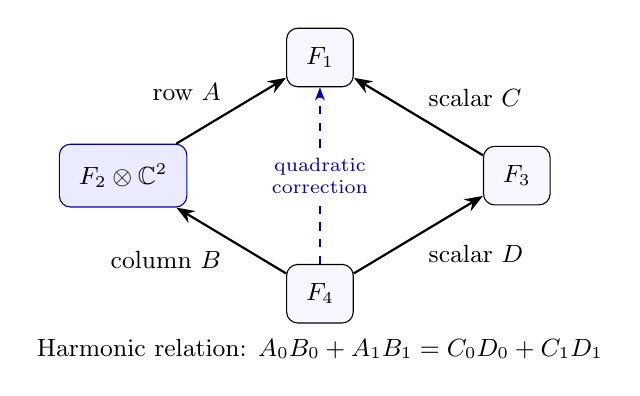
\begin{tikzpicture}[>=Stealth, every node/.style={font=\small},
 line/.style={draw,rounded corners,inner sep=7pt,fill=blue!3}]
\node[line] (one) at (0,2.7) {$F_1$};
\node[line,draw=blue!70!black,fill=blue!8] (two) at (-2.5,1.2)
 {$F_2\otimes\mathbb C^2$};
\node[line] (three) at (2.5,1.2) {$F_3$};
\node[line] (four) at (0,-.3) {$F_4$};
\draw[->,thick] (two) -- node[above left] {row $A$} (one);
\draw[->,thick] (three) -- node[above right] {scalar $C$} (one);
\draw[->,thick] (four) -- node[below left] {column $B$} (two);
\draw[->,thick] (four) -- node[below right] {scalar $D$} (three);
\draw[->,dashed,blue!70!black] (four) -- node[pos=.5,fill=white,
 inner sep=2pt,align=center,font=\scriptsize]
 {quadratic\\correction} (one);
\node at (0,-1.0) {Harmonic relation: $A_0B_0+A_1B_1=C_0D_0+C_1D_1$};
\end{tikzpicture}
\end{adjustbox}
\caption{The two composable paths in the adjacent-layer subfamily.
The repeated middle factor retains a full two-by-two matrix action.
The central correction enforces integrability after the nonzero harmonic
path classes cancel. The complete deformation space also contains the
other blocks listed in Lemma~\ref{lem:cohomology}.}
\label{fig:matrix-paths}
\end{figure}


The full harmonic deformation space $V$ has dimension $119$, including
reverse arrows and directions outside these four blocks. Its complete
obstruction has five components. For the nearby product polarizations
\eqref{eq:polarization}, let $K_p$ be the split Hodge homotopy and
$P_{2,p}$ the degree-two harmonic projection. The convergent equations
\[
 a_p(x)=\iota x-K_p(a_p(x)^2),\qquad
 \kappa_p(x)=P_{2,p}(a_p(x)^2)
\]
give the full integrability condition $\kappa_p(x)=0$.
The effective complex group is
$G=(\mathrm{GL}_1\times\mathrm{GL}_2\times\mathrm{GL}_1
\times\mathrm{GL}_1)/\CC^*$, with compact form $K$.
Its trace-free parallel algebra $\mathfrak g$ has complex dimension
six. Theorem~\ref{thm:complete-model} identifies every holomorphic
map between small reconstructed bundles with a constant harmonic
intertwiner. Thus all matrix directions, rather than only vertex
scalars, enter both the spectrum and the quotient.

Write $q_p(x)=\|\iota x\|_p^2$, where the squared norm is divided
by spatial volume. On the adjacent subspace the only quadratic
correction lies in block $14$, and all higher products vanish. The
two path obstruction classes can be nonzero and opposite, while their
sum has a nonzero coexact primitive. The family in
Section~\ref{sec:fixed-example} demonstrates this directly. It also
has a boundary kernel generated by a matrix that is not Hermitian
for $h_0$. Restricting the finite calculation to Hermitian matrix
directions would miss that complex holomorphic kernel.

\subsection{Curvature control and the actual small spectrum}
Let $b(p)$ be the centered slope differences, let $\mu_p$ be the
quadratic matrix moment map, and let $m_p$ be the remaining curvature
equation after solving on the complement of all parallel Hermitian
endomorphisms. We prove
\[
 m_p(x)=-b(p)+\mu_p(x)+R_p(x),\qquad
 |\langle\Pi,R_p(x)\rangle|
       \le Cq_p(x)q_p([\Pi,x])
\]
for every orthogonal multiplicity projection $\Pi$, including arbitrary
projections in $\CC^2$. The estimate holds on the entire ambient
ball. Its proof has two parts. Harmonic orthogonality removes the
cubic curvature terms. At a projection-preserving array, a partial
Chern--Weil identity makes the projected remainder zero, and a
reflection makes its first crossing derivative zero. Taylor's formula
then gives the crossing-energy factor.

For an integrable simple point with $\mu_p(x)=b(p)$ and small
$q=q_p(x)$, Theorem~\ref{thm:calibration} constructs a fixed-determinant
HE metric satisfying
\begin{equation}\label{eq:intro-he}
 e^{-Cq}h_0\le H\le e^{Cq}h_0.
\end{equation}
The finite correction uses a degree argument and the same crossing
factor in its positive moment increment and residual error. It does
not divide by the weakest positive orbit eigenvalue.

Let $\nu_1\le\cdots\le\nu_6$ be the eigenvalues of
$\xi\mapsto\|[\xi,\iota x]\|_p^2$ on the full complex algebra
$\mathfrak g$. For the actual trace-free endomorphism zero-form Dolbeault
eigenvalues, Lemma~\ref{lem:relative-spectrum} and
\eqref{eq:intro-he} give
\begin{equation}\label{eq:intro-spectrum}
 \left|\log\frac{\lambda_j}{\nu_j}\right|\le Cq
 \quad(\nu_j>0,\ j\le6),\qquad
 \lambda_j=0\Longleftrightarrow\nu_j=0,\qquad \lambda_7\ge\gamma>0.
\end{equation}
All constants are independent of positive eigenvalue ratios.
For the balanced family in Section~\ref{sec:balanced-family},
$q\asymp t^2$ and
$\lambda_1=\tfrac54t^2\varepsilon^2(1+O(t^2+\varepsilon^2))$,
while the other five small eigenvalues are comparable to $t^2$.
At $\varepsilon=0$ the weak mode is exactly zero and a line splits
off. We construct that nonsimple endpoint metric separately.

\subsection{The quotient and a finite-length boundary curve}
The corrected locus
$\{\kappa_p=0,m_p=0,|x|<r\}/K$ describes an open neighborhood
of actual HE classes, with uniform coverage in fixed connection norms.
Section~\ref{sec:quotient} proves compact-orbit uniqueness, identifies
the effective stabilizers, and constructs smooth locally closed complex
pieces. On these pieces Theorem~\ref{thm:quotient-metric} gives
\begin{equation}\label{eq:intro-quotient}
 (1-Cr^2)g_{\mathrm{fin},p}\le g_{\mathrm{HE},p}
                         \le(1+Cr^2)g_{\mathrm{fin},p},\qquad
 g_{\mathrm{fin},p}([v])=\inf_{\xi\in\mathfrak g}\|v-C_x\xi\|_p^2.
\end{equation}
The constant is uniform as the orbit map $C_x$ and the obstruction
derivative lose rank. The exact tangent kernel is the complex orbit
tangent. Tangents transported to the fixed subspace of the limiting
stabilizer have the specified limits in
\eqref{eq:tangent-limit-condition}. At fixed polarization, intrinsic
lengths separate points and compare on the same local path domains.

On $p_2=7p_1/5$, the piece where one copy of $F_2$ splits off
is the active stable part of the full rank-four problem of
\cite{WuebbenWallMetrics26}. We construct the change between the
two Hodge presentations and prove that their actual active tangent
metrics agree exactly. Volume normalization introduces no rank factor.

Finally, the unrotated balanced family has constant interior bundle
type. Section~\ref{sec:moving-curve} rotates a cubic into an orthogonal
polynomial direction while preserving all moment and integrability
identities. The resulting bundles are pairwise nonisomorphic, and their
actual bundle tangent has norm comparable to $t$. Including the
parameter derivative $\partial_pa_p$ and the assigned parameter metric
$|dp|^2$, we obtain
\[
 ct\varepsilon\le\operatorname{Length}_{\mathrm{act}}
      (\gamma_t|_{(0,\varepsilon]})\le Ct\varepsilon.
\]
The constants hold for independent small $t,\varepsilon$.
The curve converges to the rank-four-plus-line HE class. This is a
tail-length estimate in the stated varying-polarization space;
its lower bound is not an ambient shortest-distance bound.

\subsection{Relation to earlier work}
The qualitative local deformation theory near a fixed HE bundle,
including automorphisms and the polystability correspondence, is developed
in \cite{BuchdahlSchumacher20}. Complementary elliptic reduction and
adapted symplectic forms for varying backgrounds appear in
\cite{ClarkeTipler24,Delloque25}. We use these mechanisms with the
complete matrix kernel and verify the uniform product-domain estimates.
Our adapted form tames the complex structure; the local complex pieces
are constructed directly.

The two-step result \cite{WuebbenRepeated26} already treats repeated
stable factors, the estimate for every multiplicity projection, and
the finite degree correction. Its bipartite geometry makes the harmonic
presentation integrable without composable relations and supplies a
parity cancellation. Here we retain the full nonlinear reconstruction,
replace that cancellation by harmonic orthogonality, and treat a
nonsimple endpoint. The finite correction argument is restated and
proved in the form required by this directed matrix model.

The order of relative quotient minimization originates in
\cite{WuebbenRelativeMetrics26}. We use the general analytic formulation
and transverse linear lemma of \cite{WuebbenWallMetrics26}, after
verifying every hypothesis. The full matrix quotient, its polar
normalization, its rank-four geometric overlap, and the parameter-inclusive
moving curve are proved here. All objects remain locally free on a
fixed compact threefold; the results do not assert a matrix flow
theorem or a description of non-locally-free limits.

% Source: sections/02_complete_model.tex
\section{The complete matrix deformation model}\label{sec:model}

We first construct the local deformation problem in which the examples
will lie. Keeping the entire deformation space is necessary both for
isomorphism statements and for the quotient metric. The four composable
blocks used later form a proper subspace of this model.

\subsection{Geometry and norms}
Let $X=(\PP^1)^3$, and let $\omega_i$ be the product Fubini--Study
forms, normalized to have integral one on their factors. Set
\begin{gather}
 F_1=\cO(-2,-2,4),\quad F_2=\cO(1,-2,1),\quad
 F_3=\cO(-2,1,1),\quad F_4=\cO,\label{eq:lines}\\
 E_0=F_1\oplus(F_2\otimes\CC^2)\oplus F_3\oplus F_4,
 \qquad (m_1,m_2,m_3,m_4)=(1,2,1,1).\label{eq:split-bundle}
\end{gather}
The product Hermitian metric $h_0$ uses the standard metric on $\CC^2$.
Its connection is $A_0$ and its Dolbeault operator is $d$; the induced
operator on endomorphism forms has the same notation. Block $ij$ maps
type $j$ to type $i$. For a small real parameter $p=(p_1,p_2)$, put
\begin{equation}\label{eq:polarization}
 \omega_p=(1+p_1)^{-1}\omega_1+(1+p_2)^{-1}\omega_2+\omega_3.
\end{equation}
All Hermitian $L^2$ products are divided by
$\Vol_p=((1+p_1)(1+p_2))^{-1}$ and are linear in their second
argument. Their real parts are the associated real metrics. No norm
is divided by the bundle rank. The normalized volume measure is fixed.
Sobolev norms $H^s$, with $s\ge6$, use $\omega_0,h_0$; nearby norms
are uniformly equivalent. We fix the product determinant metric on
$\det E_0=\cO(-2,-5,7)$.
Every eigenvalue denoted $\lambda_j$ is that of the zero-form
Dolbeault Laplacian $\bar\partial_{\End_0}^*\bar\partial_{\End_0}$
on complex trace-free endomorphisms, without a factor two.
Eigenvalues are ordered with complex multiplicity, including zeros.

The contracted line curvatures and their rank-weighted average are
\begin{align}
 \kappa_1&=-4\pi(p_1+p_2),&\kappa_2&=2\pi(p_1-2p_2),\notag\\
 \kappa_3&=2\pi(-2p_1+p_2),&\kappa_4&=0,
 &\kappa_E&=-\tfrac{4\pi}{5}p_1-2\pi p_2.\label{eq:curvatures}
\end{align}
Write $b_i=\kappa_E-\kappa_i$, interpreting the second component as a
scalar matrix on $\CC^2$. Thus
\begin{equation}\label{eq:slopes}
 b(p)=\bigl(\tfrac{16\pi}{5}p_1+2\pi p_2,
 -\tfrac{14\pi}{5}p_1+2\pi p_2,
 \tfrac{16\pi}{5}p_1-4\pi p_2,
 -\tfrac{4\pi}{5}p_1-2\pi p_2\bigr).
\end{equation}
In particular $b_1+2b_2+b_3+b_4=0$ and $3b_1+2b_2+5b_4=0$.
The latter identity will determine which balanced arrays arise from
the actual polarizations \eqref{eq:polarization}.

\begin{lemma}\label{lem:cohomology}
The split trace-free cohomology dimensions in degrees zero through three
are $(6,119,5,0)$. The full degree-one space $V$ has the following blocks:
\[
\begin{array}{c|rrrrrrrrr}
ij&12&13&21&31&23&32&24&34&41\\\hline
\dim H^1(F_iF_j^{-1})&8&8&8&8&8&8&4&4&27\\
\dim V_{ij}&16&8&16&8&16&16&8&4&27.
\end{array}
\]
The only degree-two block is $14$, naturally identified with
$S_4=H^0(\PP^1_3,\cO(4))$ after choosing the two negative-factor
harmonic generators. The parallel trace-free algebra is
\begin{equation}\label{eq:parallel-algebra}
 \mathfrak g=\{(z_1,M,z_3,z_4):z_1+\tr M+z_3+z_4=0\},\qquad
 |\xi|^2=|z_1|^2+\tr(M^*M)+|z_3|^2+|z_4|^2.
\end{equation}
Here $M$ is an arbitrary complex two-by-two matrix.
\end{lemma}
\begin{proof}
The six line blocks $12,13,21,31,23,32$ have degrees obtained by
permuting $(-3,0,3)$, with one negative entry. Projective-line cohomology
and the K\"unneth formula give dimension $2\cdot1\cdot4=8$ in
degree one. Blocks $24,34$ have degrees $(1,-2,1),(-2,1,1)$ and
dimension four. Block $41$ has degrees $(2,2,-4)$ and dimension
$3\cdot3\cdot3=27$. Block $14$ has degrees $(-2,-2,4)$ and
degree-two dimension five. Blocks $42,43$ have a degree $-1$ factor
and vanish. There are no off-diagonal degree-zero or degree-three
groups. Tensoring with the multiplicity Hom spaces gives the table.
The diagonal blocks contribute $1+4+1+1$ constants and no higher
cohomology. Removing common scalars gives six constants and
\eqref{eq:parallel-algebra}. These are the standard projective-space
and product computations of \cite[Tags 01XT and 0BED]{stacks}.
\end{proof}

The effective constant groups are
\[
 G=(\mathrm{GL}_1\times\mathrm{GL}_2\times\mathrm{GL}_1
                 \times\mathrm{GL}_1)/\CC^*,\qquad
 K=(\mathrm U_1\times\mathrm U_2\times\mathrm U_1\times\mathrm U_1)/S^1.
\]
They act by $(gx)_{ij}=g_ix_{ij}g_j^{-1}$. Determinant-one lifts have
an ineffective fifth-root center. Let $\mathfrak g_{\RR}$ denote the
Hermitian part of \eqref{eq:parallel-algebra}, and write
$C_x\xi=[\xi,x]$ for the infinitesimal complex action.

The split harmonic spaces, as spaces of differential forms, are fixed
as $p$ varies. Indeed the product Laplacian is a sum of commuting
nonnegative factor Laplacians with positive coefficients
$1+p_1,1+p_2,1$. Its kernel is their common kernel. If $\iota:V\to
\Omega^{0,1}(\End_0E_0)$ is inclusion, then
\begin{align}
 q_p(x):=\|\iota x\|_p^2
 ={}&(1+p_1)(\|x_{12}\|_0^2+\|x_{32}\|_0^2+\|x_{34}\|_0^2)\notag\\
 &+(1+p_2)(\|x_{13}\|_0^2+\|x_{23}\|_0^2+\|x_{24}\|_0^2)
 +\|x_{21}\|_0^2+\|x_{31}\|_0^2+\|x_{41}\|_0^2.\label{eq:harmonic-norm}
\end{align}
The three groups have their $(0,1)$ component on the first, second and
third factors, respectively. Put $|x|^2=q_0(x)$.

Denote harmonic projections and Green operators by $P_{j,p},G_{j,p}$,
and the Hodge homotopy by $K_p=d_p^*G_p$. They have uniform bounds
between fixed Sobolev spaces and depend smoothly on $p$. To see this,
use the fixed kernels and the positive complementary gap at $p=0$;
uniform ellipticity preserves the gap and gives uniform elliptic
inverse estimates. Differentiating the inverse identity gives the
parameter derivatives. The zero-form projection $P_0$ is independent
of $p$. The degree-one projection is also independent of $p$ as an
operator: in each Hom block only the indicated differential component
pairs with a harmonic form, and both its pairing and the harmonic Gram
matrix are multiplied by the same constant in \eqref{eq:harmonic-norm}.

\subsection{Convergent reconstruction and all isomorphisms}
\begin{theorem}\label{thm:complete-model}
On a fixed product neighborhood $|p|<p_0$, $|x|<r_0$, there are maps
\begin{equation}\label{eq:reconstruction}
 a_p(x)=\iota x-K_p(a_p(x)^2),\qquad
 \kappa_p(x)=P_{2,p}(a_p(x)^2),
\end{equation}
holomorphic in $x$ and smooth in $p$. Their values are spatially smooth,
and
\begin{gather}
 \|a_p(x)-\iota x\|_{H^s}\le C|x|^2,\qquad
 \|D_xa_p(x)v-\iota v\|_{H^s}\le C|x||v|,\label{eq:reconstruction-bounds}\\
 d_p^*a_p=0,\qquad P_1a_p=x.\notag
\end{gather}
The complete equation $\kappa_p(x)=0$ is equivalent to integrability.
Every sufficiently small integrable perturbation is complex-gauge
equivalent to such a member, with uniform local gauge bounds.

Every holomorphic bundle map between two sufficiently small integrable
members at the same $p$ is a constant block matrix $g_0$ satisfying
\begin{equation}\label{eq:intertwiner}
 y_{ij}g_{0,j}=g_{0,i}x_{ij}
 \quad\hbox{in every harmonic coordinate}.
\end{equation}
Conversely every such matrix is a holomorphic map. Thus isomorphisms are
exactly the $G$ orbit relation with both coordinates in the ball.
No bound on the isomorphism or its inverse is required.
\end{theorem}
\begin{proof}
Sobolev multiplication is bounded for $s\ge6$ on this real sixfold.
The map $a\mapsto\iota x-K_p(a^2)$ is a contraction on
$\|a\|_{H^s}\le2\|\iota\||x|$ for one sufficiently small radius.
Its homogeneous series is
\[
 a_1=\iota x,\qquad
 a_n=-K_p\sum_{j=1}^{n-1}a_j\wedge a_{n-j}\quad(n\ge2).
\]
A Catalan majorant proves convergence uniformly in $p$. All matrix
products have their indicated order. Since $\tr(a\wedge a)=0$,
the reconstruction is trace-free. The Hodge identities give
$K_pa=0$, $P_1a=x$, $d_p^*a=0$. Differentiating the equation gives
\begin{equation}\label{eq:reconstruction-derivative}
 J_{p,x}v=\iota v-K_p(J_{p,x}v\wedge a_p+a_p\wedge J_{p,x}v),
 \qquad J_{p,x}=D_xa_p.
\end{equation}
The linear inverse has norm at most two after decreasing the radius.
This proves the derivative bound, and repeated differentiation proves
the fixed-order parameter estimates. The order-minus-one homotopy
and elliptic bootstrap give spatial smoothness.

For $c=da+a^2$, the Hodge and Bianchi identities give
\begin{equation}\label{eq:bianchi-reconstruction}
 c=\iota_2\kappa_p(x)+K_p(c\wedge a-a\wedge c).
\end{equation}
The last operator is small in $H^{s-1}$. Hence $\kappa_p=0$ implies
$c=0$, and the converse follows by harmonic projection.

For a small perturbation $b$, solve
$d_p^*(e^v\cdot(d+b)-d)=0$ with $v\in QH^{s+1}$, where $Q$
is the complement of all parallel complex zero-forms. The derivative
in $v$ is $-d_p^*d:QH^{s+1}\to QH^{s-1}$, a uniformly invertible
elliptic operator. The analytic implicit-function theorem gives a
local gauge with uniform bounds and first derivatives. For an
integrable Coulomb representative $b'$, Hodge decomposition gives
$b'=\iota P_1b'-K_p((b')^2)$, so contraction uniqueness identifies
it with $a_p(P_1b')$.

Every constant block matrix commutes with the split differential,
projections and homotopy. Termwise conjugation therefore proves
equivariance of each $a_n$. For a fixed $g$, summing the two convergent
series proves $a_p(gx)=ga_p(x)g^{-1}$ whenever both coordinates are
in the ball. This argument does not require the entire $g$-orbit of
the ball to stay in the ball.

Finally decompose a holomorphic map as $g=g_0+g_1$, where $g_0$ is
the full parallel projection, including scalars. Its equation is
\[
 dg_1+a_p(y)g_1-g_1a_p(x)+a_p(y)g_0-g_0a_p(x)=0.
\]
Applying $d_p^*$ kills the last two terms. Pairing with $g_1$ and
using the fixed Poincar\'e inequality gives
\[
 \|dg_1\|_p^2\le
 C(\|a_p(x)\|_\infty+\|a_p(y)\|_\infty)\|dg_1\|_p\|g_1\|_p,
 \qquad \|g_1\|_p\le C\|dg_1\|_p.
\]
Smallness forces $g_1=0$, independently of $\|g_0\|$. Harmonic
projection gives \eqref{eq:intertwiner}. Conversely that equation
intertwines every term of the ordered reconstruction series, proving
the full morphism assertion. This is the co-closed-slice mechanism
of \cite[Proposition 4.5 and Corollary 4.6]{BuchdahlSchumacher20},
with the full multiplicity algebra retained.
\end{proof}

The trace-free holomorphic endomorphisms are therefore
$\ker C_x\subset\mathfrak g$. At a nonpolystable point this complex
algebra need not be closed under the reference Hermitian adjoint.
Section~\ref{sec:fixed-example} gives an explicit instance.

\subsection{The adjacent-layer equations}
Put $S_j=H^0(\PP^1_3,\cO(j))$. On each of the first two factors
choose $e_0,e_1\in H^0(\cO(1))$, a nonzero
$\theta\in H^1(\cO(-2))$, and harmonic
$\eta^0,\eta^1\in H^1(\cO(-3))$ with
$P(\eta^je_m)=\delta_{jm}\theta$. Serre duality supplies such bases.
The $36$-dimensional adjacent-layer subspace has entries
\begin{align}
 x_{12}&=\eta_1^0A_0+\eta_1^1A_1,&A_j&\in S_3\otimes M_{1,2},\notag\\
 x_{13}&=\eta_2^0C_0+\eta_2^1C_1,&C_j&\in S_3,\notag\\
 x_{24}&=(e_{0,1}B_0+e_{1,1}B_1)\theta_2,&B_j&\in S_1\otimes M_{2,1},\notag\\
 x_{34}&=\theta_1(e_{0,2}D_0+e_{1,2}D_1),&D_j&\in S_1.\label{eq:adjacent-blocks}
\end{align}
Only block $14$ occurs in the square. Its further products with these
four blocks vanish on both sides. Consequently the restriction of the
complete model is exactly
\begin{gather}
 a_p(x)=\iota x-K_p((\iota x)^2),\label{eq:adjacent-reconstruction}\\
 \kappa_p(x)=(\theta_1\wedge\theta_2)
 (A_0B_0+A_1B_1-C_0D_0-C_1D_1).\label{eq:adjacent-obstruction}
\end{gather}
The minus sign orders the differential components by projective-line
factor. The products $A_jB_j$ are ordered row--column products, hence
scalar quartics. Their five coefficients are the complete equations on
this subspace. The full $119$-coordinate recursion can have higher terms.

% Source: sections/03_fixed_metric_example.tex
\section{A composable family at the split metric}\label{sec:fixed-example}

We begin with a family whose weak eigenvalue can be computed explicitly.
Its bundles are semistable at the equal-slope polarization and have no
Hermitian--Einstein metric there. The operator in this section uses the
fixed split metric $h_0$. Section~\ref{sec:balanced-family} constructs a
different, exactly balanced family and proves the corresponding assertion
for its actual HE metrics.

\subsection{Two nonzero compositions and their correction}
On the first two projective lines choose identical nonzero data
$\tau\in H^0(\cO(1))$, $\theta\in H^1(\cO(-2))$, and a harmonic
$\eta\in H^1(\cO(-3))$ with $P(\tau\eta)=\theta$.
Multiplication by $\tau$ on this degree-one cohomology is surjective,
dual to the injective map $H^0(\cO)\to H^0(\cO(1))$.
Put $\rho=\tau\eta$. On the third factor use homogeneous coordinates
$(s:z)$ and set $P=s^3$, $Q=z^3$, $\tau_3=s$. The cubics are
orthogonal and have equal norm. Put $c=(1,1)^T$.

For $0\le\varepsilon\le\varepsilon_0<1/2$, let $A_\varepsilon$
have precisely the four harmonic blocks
\begin{align}
 (A_\varepsilon)_{12}&=\eta_1(Pe_1^T+\varepsilon Qe_2^T),&
 (A_\varepsilon)_{13}&=\eta_2(P+\varepsilon Q),\notag\\
 (A_\varepsilon)_{24}&=\tau_1\theta_2\tau_3c,&
 (A_\varepsilon)_{34}&=\theta_1\tau_2\tau_3.\label{eq:fixed-family}
\end{align}
Suppressed tensor factors are constant sections. Its square is the
block-$14$ two-form
\begin{equation}\label{eq:fixed-curvature}
 W_\varepsilon=(\rho_1\wedge\theta_2-\theta_1\wedge\rho_2)
                  \tau_3(P+\varepsilon Q).
\end{equation}
It is closed and has zero harmonic projection. With the reference
homotopy $K_0$, set
\begin{equation}\label{eq:fixed-integrable}
 \Gamma_\varepsilon=-K_0W_\varepsilon,\qquad
 N_{t,\varepsilon}=tA_\varepsilon+t^2\Gamma_\varepsilon E_{14},
 \qquad 0<t<t_0.
\end{equation}
The notation $E_{14}$ here records the block of the scalar form.

\begin{proposition}\label{prop:fixed-integrable}
The operators $d+N_{t,\varepsilon}$ are integrable and co-closed and
are the complete reconstructions of $x=tA_\varepsilon$.
Both ordered composition classes are nonzero and opposite, and
$\Gamma_\varepsilon\ne0$. Every fixed spatial norm of $N$ is $O(t)$,
uniformly in the stated parameter rectangle.
\end{proposition}
\begin{proof}
Product Hodge theory gives $P_2W_\varepsilon=0$ from
$P\rho=\theta$. The Hodge identity gives
$d\Gamma_\varepsilon=-W_\varepsilon$, $d^*\Gamma_\varepsilon=0$,
and $P_1\Gamma_\varepsilon=0$. Every product of block $14$ with
the active blocks vanishes. Thus $dN+N^2=0$ and
$N=\iota x-K_0(N^2)$ exactly.

The form $\theta$ is nowhere zero as a smooth section of
$\Lambda^{0,1}\otimes\cO(-2)$: its Serre-dual section is a nonzero
constant. The form $\rho$ vanishes at the zero of $\tau$ and has
nonzero harmonic projection. Hence $\rho,\theta$ are linearly
independent, so $W_\varepsilon\ne0$ and its primitive is nonzero.
Each path has class, up to sign,
$\theta_1\wedge\theta_2\tau_3(P+\varepsilon Q)\ne0$.
The forms depend affinely on $\varepsilon$, and the fixed Green
operator has bounded action in every fixed smooth order; this proves
the norm assertion.
\end{proof}

Replacing only the
scalar route by $P+\varepsilon Q+\delta R$, with nonzero $R\in S_3$,
leaves harmonic curvature
$-t^2\delta\theta_1\wedge\theta_2\tau_3R$. No choice of a central
block-$14$ primitive can remove this class with the four harmonic
arrows fixed.

\subsection{Noncommutation, stabilizers and bundle type}
Up to positive norm constants, the multiplicity contractions in the
row and column data are
\begin{equation}\label{eq:fixed-commutator}
 U_\varepsilon=\begin{pmatrix}1&0\\0&\varepsilon^2\end{pmatrix},
 \qquad V=\begin{pmatrix}1&1\\1&1\end{pmatrix},\qquad
 [U_\varepsilon,V]=(1-\varepsilon^2)
                 \begin{pmatrix}0&1\\-1&0\end{pmatrix}.
\end{equation}
They cannot be simultaneously diagonalized by a unitary multiplicity
basis. In particular the scalar vertex graph omits relevant directions.

\begin{proposition}\label{prop:fixed-centralizer}
For $t>0$ and $\varepsilon>0$, the full holomorphic endomorphism algebra
is scalar. At $\varepsilon=0$ it is
\begin{equation}\label{eq:fixed-centralizer}
 z_1=z_3=z_4=s_0,\qquad
 M=\begin{pmatrix}s_0&0\\s_0-n&n\end{pmatrix},\qquad s_0,n\in\CC.
\end{equation}
The bundle then splits as a rank-four three-step extension and one copy
of $F_2$, with effective automorphism group $\CC^*$. The trace-free
kernel is generated by
\begin{equation}\label{eq:fixed-kernel}
 \Xi=(1,M_0,1,1),\qquad M_0=\begin{pmatrix}1&0\\5&-4\end{pmatrix},
 \qquad |\Xi|^2=45.
\end{equation}
All these bundles, for $t>0$, are semistable but not polystable at
$\omega_0$. They have no HE metric at that polarization.
\end{proposition}
\begin{proof}
By Theorem~\ref{thm:complete-model}, it suffices to compute constant
intertwiners. At positive $\varepsilon$, the two independent cubic
coefficients in block $12$ force both rows of $M$ to equal those of
$z_1I_2$. The other scalar arrows force $z_3=z_4=z_1$.
At zero, only the first row is fixed; the column equation $Mc=s_0c$
gives \eqref{eq:fixed-centralizer}. Its trace is $4s_0+n$, giving
\eqref{eq:fixed-kernel}. In the multiplicity basis $(c,e_2)$ the
centralizer is diagonal. The column uses the first basis vector, and
the row annihilates the second, which splits off the stated $F_2$.
The active rank-four part retains both paths and their correction.

The three-step filtration has slope-zero polystable quotients and
refines to a filtration by the four line types. Hence it is semistable
and has graded object $E_0$. If it were polystable, it would be
isomorphic to that graded object. Its endomorphism algebra would then
have dimension seven, whereas the computed dimensions are one and two.
Thus it is not polystable. The HE-to-polystable implication
\cite[Theorem 5.8.3]{Kobayashi87} rules out an HE metric.
\end{proof}

For fixed $\varepsilon$, changing $t>0$ stays on one holomorphic
orbit: the determinant-one gauge of weights $(1,0,0,-1)$ on the
four types scales every adjacent block by $t$ and the central one
by $t^2$. Different $\varepsilon$ give different bundles over the
fixed base, since the ratio of the $P,Q$ coefficients in scalar
block $13$ is invariant. These are distinct holomorphic isomorphism
classes with the same polystable graded object. The composable route
$4\to2\to1$ also shows that this is not a two-layer presentation
with each of these fixed stable types assigned to a single layer.

\subsection{The weak eigenvalue}
Let the fixed squared harmonic norms be
\[
 a=\|\eta_1P\|_0^2=\|\eta_1Q\|_0^2
  =\|\eta_2P\|_0^2=\|\eta_2Q\|_0^2,\qquad
 b=\|\tau_1\theta_2\tau_3\|_0^2
  =\|\theta_1\tau_2\tau_3\|_0^2.
\]
Orthogonality of the cubics and blocks makes the full finite form
$t^2Q_\varepsilon$, where, on \eqref{eq:parallel-algebra},
\begin{align}
 Q_\varepsilon(\xi)={}&a\bigl(
 \|z_1e_1^T-e_1^TM\|^2+
 \varepsilon^2\|z_1e_2^T-e_2^TM\|^2+
 (1+\varepsilon^2)|z_1-z_3|^2\bigr)\notag\\
 &+b\bigl(\|Mc-cz_4\|^2+|z_3-z_4|^2\bigr).
 \label{eq:fixed-finite-form}
\end{align}
Let $\mu_1\le\cdots\le\mu_6$ be its eigenvalues with the
complex inner product \eqref{eq:parallel-algebra}, counting zeros.

\begin{lemma}\label{lem:fixed-weak}
For a sufficiently small fixed $\varepsilon_0$,
\[
 \mu_1(\varepsilon)=\tfrac{10a}{9}\varepsilon^2+O(\varepsilon^4),
 \qquad c\le\mu_j(\varepsilon)\le C\quad(2\le j\le6).
\]
\end{lemma}
\begin{proof}
At zero the kernel is $\CC\Xi$ and its complement has a positive
gap. The form depends affinely on $e=\varepsilon^2$. On the unit
kernel vector the coefficient of $e$ is
\[
 \frac a{45}\|e_2^T-e_2^TM_0\|^2
 =\frac a{45}\|(-5,5)\|^2=\frac{10a}{9}.
\]
With respect to $\CC\Xi\oplus\Xi^\perp$, the operator is
\[
 \begin{pmatrix}e(10a/9)&eB^*\\eB&L_\perp+eC\end{pmatrix}.
\]
Min--max isolates one small eigenvalue while keeping the other five
in a fixed positive interval. The scalar Schur equation for that
eigenvalue $\lambda$ is
$\lambda=e(10a/9)-e^2B^*(L_\perp+eC-\lambda)^{-1}B$.
The inverse is uniformly bounded, proving the expansion.
\end{proof}

\begin{corollary}\label{thm:fixed-spectrum}
Let $\lambda_j(t,\varepsilon)$ be the eigenvalues, with complex
multiplicity and counting zeros, of the trace-free endomorphism zero-form
Dolbeault Laplacian for $d+N_{t,\varepsilon}$, $h_0,\omega_0$.
The operator is $\bar\partial^*\bar\partial$ without a factor two.
Uniformly for independent $0<t<t_0$, $0<\varepsilon\le\varepsilon_0$,
\begin{gather}
 \lambda_1=\tfrac{10a}{9}t^2\varepsilon^2
                  (1+O(\varepsilon^2+t^2)),\label{eq:fixed-weak-law}\\
 ct^2\le\lambda_j\le Ct^2\quad(2\le j\le6),\qquad
 \lambda_7\ge\gamma>0,\notag\\
 \left|\log\frac{\lambda_j}{t^2\mu_j(\varepsilon)}\right|
 \le Ct^2\quad(1\le j\le6).\notag
\end{gather}
At $\varepsilon=0$ there is exactly one trace-free zero mode; the
five positive-mode estimates and the seventh gap persist.
\end{corollary}
\begin{proof}
Proposition~\ref{prop:fixed-integrable} gives an integrable, co-closed
reconstruction with $\|N\|_\infty\le Ct$ and
$q_0(x)=t^2\{2a(1+\varepsilon^2)+3b\}$. The relative spectral
lemma proved in Section~\ref{subsec:spectral-reduction} compares all
six eigenvalues to the full finite form with relative error $O(t^2)$,
including exact kernels and a seventh gap. Combine it with
Lemma~\ref{lem:fixed-weak}. No inverse of $\mu_1$ is used, so there
is no condition on the ratio of $t$ and $\varepsilon$.
\end{proof}

% Source: sections/04_projection_calibration.tex
\section{Multiplicity projections and the HE correction}\label{sec:calibration}

Quadratic balance determines a useful reference metric, but does not
solve the nonlinear HE equation. The correction must be controlled even
when the finite matrix action has very small positive eigenvalues.
The required estimate pairs the curvature error with every orthogonal
projection in every multiplicity space. The proof uses harmonic
orthogonality to eliminate cubic terms; it applies to the complete
deformation space, which contains reverse arrows and higher products.

\subsection{The ambient complementary equation}
Let $P_0$ project the trace-free Hermitian zero-forms onto
$\mathfrak g_{\RR}$, and put $Q_0=1-P_0$. For $u\in Q_0H^{s+1}$,
form the connection compatible with $d+a_p(x)$ and $h_0e^u$, and
transport it to $h_0$ by $e^{u/2}$. Denote that unitary connection by
$\Phi(p,x,u)$ and its centered contracted curvature by
\begin{equation}\label{eq:mean-curvature}
 \mathcal M(p,x,u)=i\Lambda_pF_{\Phi(p,x,u)}-\kappa_E(p)I.
\end{equation}
The connection is defined off the integrable locus as well. Its fixed
determinant has constant mean curvature, so $\mathcal M$ is pointwise
trace-free.

\begin{lemma}\label{lem:complement}
On one uniform product neighborhood there is a unique small solution
$u(p,x)\in Q_0H^{s+1}$ of
\begin{equation}\label{eq:complement}
 Q_0\mathcal M(p,x,u(p,x))=0,
 \qquad \|u(p,x)\|_{H^{s+1}}\le C|x|^2,
 \qquad \|D_xu(p,x)v\|_{H^{s+1}}\le C|x||v|.
\end{equation}
It is smooth in $p,x$, equivariant under $K$, and has uniform
fixed-order spatial and parameter estimates on smaller neighborhoods.
\end{lemma}
\begin{proof}
At $x=u=0$, $\mathcal M=-b(p)$ is parallel. The derivative in the
real Hermitian metric variable, including the unitary transport, is
\begin{equation}\label{eq:metric-linearization}
 L_p=\tfrac12(\Delta_{\bar\partial,p}+\Delta_{\partial,p}),\qquad
 \langle u,L_pu\rangle_p=\tfrac12
       (\|\bar\partial u\|_p^2+\|\partial u\|_p^2).
\end{equation}
Indeed the curvature derivative of $h_0e^u$ is the contracted
$\bar\partial\partial$ term, and differentiating the transport
adds half its curvature commutator; the K\"ahler identities give
the symmetric average in \eqref{eq:metric-linearization}. The kernel
on Hermitian fields is the full parallel algebra. The uniform split
gap and ellipticity give an inverse
$Q_0H^{s-1}\to Q_0H^{s+1}$. The parameter implicit-function theorem
therefore gives a smooth solution with $u(p,0)=0$.

The linear curvature variation in $x$ vanishes by harmonicity and
the K\"ahler identities. Hence $D_xu(p,0)=0$, proving the estimates
by Taylor's formula. Elliptic regularity and differentiated equations
give the higher bounds. Uniqueness proves $K$-equivariance. This is
the complementary reduction of \cite[Section 3]{ClarkeTipler24}
and \cite[Lemma 4.1 and Proposition 4.2]{Delloque25}, on a fixed
Sobolev complement containing the entire matrix kernel.
\end{proof}

Set $H_x=h_0e^{u(p,x)}$, $\Phi_p(x)=\Phi(p,x,u(p,x))$ and
$m_p(x)=P_0\mathcal M(p,x,u(p,x))$. At an integrable point,
$m_p(x)=0$ is exactly the remaining HE equation. Define the quadratic
moment map by the real trace pairing
\begin{equation}\label{eq:moment}
 \langle\xi,\mu_p(x)\rangle
 =\langle[\xi,\iota x],\iota x\rangle_p
 =\left.\frac{d}{dt}\right|_{t=0}q_p(e^{t\xi/2}\cdot x),
 \qquad \xi\in\mathfrak g_{\RR}.
\end{equation}
It is incoming $xx^*$ minus outgoing $x^*x$, with the current harmonic
Gram forms. Both $m_p$ and $\mu_p$ are in the full six-dimensional
Hermitian algebra. Write
\begin{equation}\label{eq:residual}
 m_p(x)=-b(p)+\mu_p(x)+R_p(x).
\end{equation}

\subsection{Quartic order and every projection}
\begin{lemma}\label{lem:quartic}
On the entire ambient ball,
\[
 |R_p(x)|\le C|x|^4,\qquad
 \|D_xR_p(x)\|\le C|x|^3,\qquad
 \|D_x^2R_p(x)\|\le C|x|^2.
\]
The constants are uniform in $p$.
\end{lemma}
\begin{proof}
Let $\alpha=\Phi_p(x)^{0,1}-d$. The transformation rule gives
\[
 \alpha=e^{u/2}a_pe^{-u/2}-(de^{u/2})e^{-u/2}
       =\iota x+B+O(|x|^3),\qquad
 B=a_p-\iota x-\tfrac12du.
\]
Here $B=O(|x|^2)$ and is orthogonal to every current harmonic
one-form: its first summand is coexact and its second exact.
The linear curvature term, integrated against a parallel Hermitian
matrix, vanishes by integration by parts. The exact remaining identity is
\begin{equation}\label{eq:integrated-moment}
 \langle\xi,m_p(x)\rangle
 =-\langle\xi,b(p)\rangle+\langle[\xi,\alpha],\alpha\rangle_p.
\end{equation}
Parallel left and right multiplication preserve the harmonic subspace.
Consequently both cubic cross terms between $\iota x$ and $B$ vanish.
The remaining difference from \eqref{eq:moment} is $O(|x|^4)$.
The argument holds for every ambient $x$, so all Taylor coefficients
of $R_p$ of degree below four vanish. Its smoothness and uniform
fourth-derivative bound give the two derivative estimates.
\end{proof}

An orthogonal multiplicity projection means a tuple
$\Pi=(\Pi_1,\Pi_2,\Pi_3,\Pi_4)$ with
$\Pi_i^2=\Pi_i=\Pi_i^*$ on $\CC^{m_i}$. It need not be diagonal
in the fixed basis of $\CC^2$. Since $R_p$ has total trace zero,
its trace pairing with $\Pi$ is defined without imposing a trace
condition on $\Pi$.

\begin{proposition}\label{prop:projection-residual}
For every such projection and every sufficiently small ambient array,
\begin{equation}\label{eq:projection-residual}
 |\langle\Pi,R_p(x)\rangle|
 \le Cq_p(x)q_p([\Pi,x]).
\end{equation}
This includes nonintegrable arrays and all ranks and directions of
the multiplicity projections.
\end{proposition}
\begin{proof}
Decompose $x=A+C$ into the preserving and crossing blocks of $\Pi$:
\[
 A_{ij}=\Pi_ix_{ij}\Pi_j+(1-\Pi_i)x_{ij}(1-\Pi_j),\qquad C=x-A.
\]
These parts are orthogonal for every harmonic Gram form. Thus
$q_p(A+sC)\le q_p(x)$ for $0\le s\le1$ and
$q_p(C)=q_p([\Pi,x])$.

At $C=0$, the circle generated by $\Pi$ fixes $A$. Equivariance
of reconstruction and uniqueness in Lemma~\ref{lem:complement}
make the compatible connection preserve
$E_\Pi=\bigoplus_iF_i\otimes\im\Pi_i$ and its complement.
The integrated trace of its curvature on $E_\Pi$ is topological:
\[
 \Vol_p^{-1}\int_X\tr\bigl(\Pi i\Lambda_pF\bigr)dV_p
 =\sum_i\rk(\Pi_i)\kappa_i.
\]
This Chern--Weil identity applies to any compatible connection on
the preserved smooth bundle, including a nonintegrable one.
Also $[\Pi,A]=0$, so $\langle\Pi,\mu_p(A)\rangle=0$.
It follows that $\langle\Pi,R_p(A)\rangle=0$.

The unitary reflection $2\Pi-I$ fixes $A$ and sends $C$ to $-C$.
Compact equivariance makes the scalar function
$C\mapsto\langle\Pi,R_p(A+C)\rangle$ even, so its first derivative
at zero vanishes. Taylor's integral formula and Lemma~\ref{lem:quartic}
now give
\[
 |\langle\Pi,R_p(A+C)\rangle|
 \le Cq_p(x)\|C\|_p^2.
\]
All projections have norm at most $\sqrt5$ and range over a finite
union of compact Grassmannians. The same constant therefore works
for all of them, proving \eqref{eq:projection-residual}.
\end{proof}

The projection method and the finite degree argument below come from
the two-step repeated-factor analysis in \cite{WuebbenRepeated26}.
The new analytic point here is the quartic cancellation on the complete
composable model: a two-step sign symmetry is unavailable in the presence
of its reverse arrows. The preserving arrays in the proof were not
required to satisfy the nonlinear relations.

\subsection{The finite correction without a spectral lower bound}
We give the finite argument in the normalization needed here. Fix a
matrix representation with total multiplicity $M\ge2$ and positive
Hermitian arrow Gram forms, allowing mixing only among coordinates
with the same ordered endpoints. Let $q$ be its squared norm and
$\mu$ its moment map as in \eqref{eq:moment}. The Hermitian domain
and target both have total trace zero.

\begin{lemma}\label{lem:finite-correction}
Suppose $\mu(Z)=b$, the complex centralizer of $Z$ is the common
scalars, and $\sigma=q(Z)>0$. Let $R$ be continuous at all
$e^{Y/2}\cdot Z$ with $Y=Y^*$, $\tr Y=0$, $\|Y\|_{\op}\le a_0$.
Assume there that
$|\langle\Pi,R(W)\rangle|\le Cq(W)q([\Pi,W])$ for every
multiplicity projection. For sufficiently small $\sigma$ there is
$Y$ with $\|Y\|_{\op}\le A\sigma$ such that
\[
 \mu(e^{Y/2}\cdot Z)-b+R(e^{Y/2}\cdot Z)=0.
\]
The constants depend on $C,M,a_0$ and the fixed norm conventions,
uniformly over a relatively compact set of positive arrow Gram forms.
\end{lemma}
\begin{proof}
Consider
$H_s(Y)=\mu(e^{Y/2}\cdot Z)-b+sR(e^{Y/2}\cdot Z)$,
$0\le s\le1$, on $\|Y\|_{\op}<a=A\sigma$.
Take $a<\min(1,a_0)$. On its boundary diagonalize every block of
$Y$ and sort all $M$ eigenvalues, keeping their vertex labels.
Trace zero implies an oscillation at least $a$, so an adjacent gap
$\delta$ is at least $a/(M-1)$. Let $\Pi$ project onto the
eigenvectors above that gap.

Whiten arrow coordinates for each ordered pair of vertices. This
commutes with the vertex action. Let $w_{ij}$ be the sum of squared
entries from source eigenvector $j$ to target eigenvector $i$.
The positive gauge multiplies these weights by $e^{y_i-y_j}$.
Using balance at $Z$ gives
\begin{align}
 \langle\Pi,\mu(e^{Y/2}\cdot Z)-b\rangle
 &=\sum_{i,j}(\Pi_i-\Pi_j)(e^{y_i-y_j}-1)w_{ij}\notag\\
 &\ge(1-e^{-\delta})q([\Pi,Z])
 \ge e^{-2a}\frac{a}{M-1}q([\Pi,Z]).\label{eq:finite-boundary}
\end{align}
Both crossing orientations contribute positively. The crossing energy
is positive because $\Pi$ is nonscalar and the centralizer is scalar.
Writing $W=e^{Y/2}\cdot Z$, the gauge bounds give
$q(W)\le e^{2a}\sigma$ and
$q([\Pi,W])\le e^{2a}q([\Pi,Z])$. Hence the residual pairing is
at most $Ce^{4a}\sigma q([\Pi,Z])$.
Choose $A>2C(M-1)$ and then $\sigma$ small enough that
$e^{6A\sigma}<2$. The positive term in \eqref{eq:finite-boundary}
strictly dominates the error. No $H_s$ has a boundary zero.
The projection is chosen pointwise; its continuity is unnecessary.

To compute the degree at $s=0$, fix nonzero $Y$ and set
$f(t)=q(e^{tY/2}\cdot Z)-t\langle b,Y\rangle$. Then $f'(0)=0$ and
\[
 f''(t)=\sum_{i,j}(y_i-y_j)^2e^{t(y_i-y_j)}w_{ij}>0.
\]
Equality would make $Y$ a scalar centralizer element, and trace zero
would force $Y=0$. Thus $\langle Y,H_0(Y)\rangle=f'(1)>0$.
The radial homotopy from $H_0$ to the identity has no boundary zero,
so its Brouwer degree is $+1$. Homotopy invariance through $H_s$
gives a zero of $H_1$ inside the ball.
\end{proof}

\begin{theorem}\label{thm:calibration}
There are uniform $p_0,r,C>0$ such that the following holds.
Suppose $|p|<p_0$, $\kappa_p(x)=0$, $\ker C_x=0$ in the
trace-free complex algebra, $\mu_p(x)=b(p)$, and
$0<q_p(x)<r^2$. Then $d+a_p(x)$ has a fixed-determinant HE metric
$H$ satisfying
\begin{equation}\label{eq:he-comparison}
 e^{-Cq_p(x)}h_0\le H\le e^{Cq_p(x)}h_0.
\end{equation}
The bundle is stable. The constant is independent of all positive
singular values of $C_x$ and their ratios.
\end{theorem}
\begin{proof}
Choose a fixed positive-gauge radius $a_0$. Decrease $r$ so that
every $e^{Y/2}x$ in that gauge ball remains in the ambient domain of
Proposition~\ref{prop:projection-residual}. Its bound verifies every
hypothesis of Lemma~\ref{lem:finite-correction}, with $M=5$.
We obtain $\|Y\|_{\op}\le Cq_p(x)$ and
$x'=e^{Y/2}\cdot x$ with $m_p(x')=0$. Exact equivariance preserves
integrability. The complementary and finite curvature equations now
both vanish, so $h_0e^{u(p,x')}$ is HE on $d+a_p(x')$.

Pull back by the constant holomorphic isomorphism $g=e^{Y/2}$.
In an $h_0$-unitary frame the resulting metric has matrix
$g^*e^{u(p,x')}g$. Since
$q_p(x')\le e^{2\|Y\|_{\op}}q_p(x)$, Lemma~\ref{lem:complement}
and Hermitian-form order give \eqref{eq:he-comparison}.
This uses no commutation between $u$ and $Y$.
Both are trace-free, so the determinant metric is preserved.
An HE bundle is polystable; its scalar endomorphism algebra permits
only one stable summand, proving stability.
\end{proof}

The theorem supplies a pointwise small correction. It neither asserts a
uniform derivative for a chosen balancing gauge nor characterizes every
stable orbit by a small quadratically balanced representative. The full
local HE quotient is constructed in Section~\ref{sec:quotient} from the
corrected equation $m_p=0$ itself. Reverse arrows allow cancellation in
$\mu_p$, so small $b(p)$ alone does not control $q_p(x)$.

% Source: sections/05_balanced_spectrum.tex
\section{Actual HE metrics and all six small modes}\label{sec:balanced-family}

The full matrix algebra gives six small complex eigenvalues. We first
compare them to the finite commutator form, retaining exact zeros.
We then construct a balanced family for which one positive eigenvalue
vanishes at a nonsimple endpoint. The endpoint metric is obtained by
a separate correction on its active summand.

\subsection{Relative spectral reduction}\label{subsec:spectral-reduction}
For a complete integrable reconstruction $N=a_p(x)$ define
\begin{equation}\label{eq:finite-spectrum}
 \cQ_{p,x}(\xi)=\|[\xi,\iota x]\|_p^2,\qquad
 0\le\nu_1(p,x)\le\cdots\le\nu_6(p,x),
 \quad \xi\in\mathfrak g,
\end{equation}
using the full complex norm \eqref{eq:parallel-algebra}.

\begin{lemma}\label{lem:relative-spectrum}
There are uniform $r,C,\gamma>0$ such that, when
$\kappa_p(x)=0$ and $q=q_p(x)<r^2$, the zero-form Dolbeault
eigenvalues on $\End_0E_0$ for $d+N$ with metric $h_0$ satisfy
\begin{equation}\label{eq:relative-spectrum}
 \lambda_j=0\ \Longleftrightarrow\ \nu_j=0,\qquad
 \left|\log\frac{\lambda_j}{\nu_j}\right|\le Cq
 \quad(\nu_j>0,\ 1\le j\le6),\qquad \lambda_7\ge\gamma.
\end{equation}
The same statement holds for any bundle metric $H$ with
$e^{-C_0q}h_0\le H\le e^{C_0q}h_0$, with constants also depending
on $C_0$. The split slopes need not be equal.
\end{lemma}
\begin{proof}
Parallel complex endomorphisms commute with the split Hodge operators.
Commuting \eqref{eq:reconstruction} with $\xi$ gives
\[
 \|[N-\iota x,\xi]\|_p
 \le C\|N\|_\infty\|[N,\xi]\|_p
 \le C\sqrt q\,\|[N,\xi]\|_p.
\]
The harmonic part and the coexact remainder are orthogonal. Thus, with
$q_N(\xi)=\|[N,\xi]\|_p^2$,
\begin{equation}\label{eq:commutator-comparison}
 \cQ_{p,x}\le q_N\le(1-Cq)^{-1}\cQ_{p,x},
 \qquad \ker q_N=\ker\cQ_{p,x}.
\end{equation}

Let $D_N=d+[N,\cdot]$ and let $\eta$ be the $L^2$ operator norm
of multiplication by $[N,\cdot]$; then $\eta\le C\sqrt q$.
If $\gamma_0$ is the uniform split zero-form gap, put
$\gamma_N=(\sqrt{\gamma_0}-\eta)^2$. On the complement
$\mathfrak g^\perp\subset L^2(\End_0E_0)$,
$\|D_Nv\|_p^2\ge\gamma_N\|v\|_p^2$.
Co-closedness implies $\langle[N,\xi],dv\rangle_p=0$ for every
parallel $\xi$. Expanding the square and applying Young's inequality
therefore yields
\begin{equation}\label{eq:spectral-block-lower}
 \|D_N(\xi+v)\|_p^2
 \ge(1-2\eta^2/\gamma_N)q_N(\xi)
          +\tfrac12\gamma_N\|v\|_p^2.
\end{equation}
For example, bound the cross term by
$2\eta\sqrt{q_N(\xi)}\|v\|_p$ and absorb half the complementary
lower bound. The trial space $\mathfrak g$ gives the upper bounds
by the eigenvalues of $q_N$. The block diagonal lower form in
\eqref{eq:spectral-block-lower} gives the matching bounds for all
six eigenvalues, after shrinking $q$ so their upper bounds lie below
$\gamma_N/2$. The codimension-six complementary inequality gives the
seventh gap. Combining with \eqref{eq:commutator-comparison} proves
\eqref{eq:relative-spectrum}. Its ingredients are parallelness,
co-closedness and the split gap, all valid at unequal slopes.

Finally the Hermitian-form inequality for $H$ changes both numerator
and denominator in each endomorphism Rayleigh quotient by factors
$e^{\pm2C_0q}$. Min--max changes every positive eigenvalue by at most
$e^{\pm4C_0q}$ and preserves the gap. The kernel is holomorphic and
independent of the metric, giving the zero assertion as well.
\end{proof}

This is the relative Kuranishi spectral argument applied to the full
parallel algebra. We included its proof to verify the unequal-slope
case and the precise zero convention. For the metrics constructed in
Theorem~\ref{thm:calibration}, the lemma gives all six HE eigenvalues
with error $O(q_p(x))$, independently of their positive ratios.

\subsection{An explicitly balanced family}
Use the forms $\eta,\theta,\tau$ from Section~\ref{sec:fixed-example}.
Rescale the orthogonal coordinate cubics $P,Q$ together and rescale
$\tau_3$ separately so that
\begin{equation}\label{eq:balanced-normalization}
 \|\eta_1P\|_0^2=\|\eta_1Q\|_0^2
 =\|\eta_2P\|_0^2=\|\eta_2Q\|_0^2
 =\|\tau_1\theta_2\tau_3\|_0^2
 =\|\theta_1\tau_2\tau_3\|_0^2=1.
\end{equation}
These two rescalings preserve $P(\tau\eta)=\theta$ and the
composition identities. For independent $0<t<t_0$ and
$0\le\varepsilon\le\varepsilon_0<1/2$, set
\begin{gather}
 e=\varepsilon^2,\qquad
 z(e)=\frac{4e-2+\sqrt{64+44e+16e^2}}{10},\qquad
 T=\frac{t^2}{18\pi},\label{eq:balanced-z}\\
 A=e+1+z,\qquad B=-2e+7(1+z),\qquad
 \beta=(1-TB)^{-1},\notag\\
 p_2=\beta-1,\qquad
 p_1=5T\beta A,\qquad \alpha=1+p_1,\label{eq:balanced-parameters}\\
 D=\frac\beta\alpha z,\qquad
 L=\sqrt{\frac\beta\alpha}\,\frac1{\sqrt2}
 \begin{pmatrix}\sqrt{1+e}&\varepsilon\\
                 \sqrt{1+e}&-\varepsilon\end{pmatrix}.
 \label{eq:balanced-rows}
\end{gather}
Here $z$ is a positive scalar function, and $A,B$ are scalar
auxiliary functions. The homogeneous third-factor coordinate no longer
appears in these formulas. We have
\begin{equation}\label{eq:z-identity}
 z(0)=\tfrac35,\qquad 5z^2+(2-4e)z-3-3e=0.
\end{equation}
For a fixed small $t_0$, the denominator $1-TB$ exceeds $1/2$;
$\alpha,\beta,D$ are positive, $|p|=O(t^2)$, and
$\alpha,\beta=1+O(t^2)$ uniformly on the whole rectangle.

Let $\ell_P,\ell_Q$ be the rows of $L$ and put
\[
 C_{t,\varepsilon}=\frac{P\ell_Pe_1+Q\ell_Qe_1}{\sqrt D}
                  =\sqrt{\frac{1+e}{2z}}(P+Q).
\]
Define $x=t\mathcal A_{t,\varepsilon}$ by
\begin{align}
 \mathcal A_{12}&=\eta_1(P\ell_P+Q\ell_Q),&
 \mathcal A_{13}&=\eta_2C_{t,\varepsilon},\notag\\
 \mathcal A_{24}&=\tau_1\theta_2\tau_3e_1,&
 \mathcal A_{34}&=\theta_1\tau_2\tau_3\sqrt D,
 \label{eq:balanced-family}
\end{align}
with every other harmonic block zero.

\begin{proposition}\label{prop:balanced-family}
The tuple \eqref{eq:balanced-family} satisfies the complete
integrability equation and $\mu_p(x)=b(p)$ at its stated polarization.
Its reconstruction is
\begin{equation}\label{eq:balanced-reconstruction}
 N=t\mathcal A_{t,\varepsilon}-t^2K_pW_{t,\varepsilon}E_{14},
\end{equation}
where
\begin{equation}\label{eq:balanced-square}
 W_{t,\varepsilon}=(\rho_1\wedge\theta_2-\theta_1\wedge\rho_2)
 \tau_3\sqrt{\frac{\beta(1+e)}{2\alpha}}(P+Q)\ne0.
\end{equation}
Its full centralizer is scalar for $\varepsilon>0$. At zero it is
\begin{equation}\label{eq:balanced-centralizer}
 z_1=z_3=z_4=s_0,\qquad M=\diag(s_0,n).
\end{equation}
The energy is
\begin{equation}\label{eq:balanced-energy}
 q_p(x)=t^2\beta\left(2+2e+\frac{1+e}{z}+z\right)\asymp t^2.
\end{equation}
\end{proposition}
\begin{proof}
The defining identity for $C_{t,\varepsilon}$ makes the two ordered
path products have opposite nonzero harmonic classes. Their sum is
\eqref{eq:balanced-square}, a nonzero exact form by the same
$\rho,\theta$ argument as before. All further products with block
$14$ vanish, proving \eqref{eq:balanced-reconstruction} and exact
integrability.

Since $L^*L=(\beta/\alpha)\diag(1+e,e)$, the moment of the
unscaled tuple is
\begin{equation}\label{eq:balanced-moment}
 \mu_p(\mathcal A)=\beta\left(
 1+2e+\frac{1+e}{z},\ -eI_2,\ z-\frac{1+e}{z},\ -1-z\right).
\end{equation}
In particular the incoming and outgoing multiplicity contractions
differ by the scalar $-\beta eI_2$. The weighted total trace is
zero, and \eqref{eq:z-identity} gives the second relation
$3\mu_1+2\mu_2+5\mu_4=0$. Directly from
\eqref{eq:balanced-parameters}, using $B-7A=-9e$ and
$2A+B=9(1+z)$,
\[
 b_2(p)=-t^2\beta e,\qquad b_4(p)=-t^2\beta(1+z).
\]
The two linear relations determine the remaining entries, proving
$\mu_p(x)=b(p)$. Summing the four squared block norms gives
\eqref{eq:balanced-energy}.

At positive $\varepsilon$ the two rows of $L$ are independent, and
the independent cubic coefficients force $M=z_1I_2$ in any constant
intertwiner. The other arrows force all scalar entries to agree.
At zero the rows and the column use only $e_1$, giving
\eqref{eq:balanced-centralizer}. Theorem~\ref{thm:complete-model}
identifies these with the full holomorphic endomorphisms.
\end{proof}

The aggregate moment is scalar at the repeated vertex, but its individual
contractions do not commute. For $U_P=\ell_P^*\ell_P$ and
$V=e_1e_1^*$,
\begin{equation}\label{eq:balanced-commutator}
 [U_P,V]=\frac\beta{2\alpha}
 \begin{pmatrix}0&-\varepsilon\sqrt{1+e}\\
                 \varepsilon\sqrt{1+e}&0\end{pmatrix}\ne0
 \quad(\varepsilon>0).
\end{equation}
This is compatible with exact matrix balance. The family is used here
for calibration and spectral degeneration; its interior isomorphism
type will be discussed in Section~\ref{subsec:isotrivial}.

\subsection{The nonsimple endpoint and its weak mode}
\begin{theorem}\label{thm:balanced-spectrum}
Every tuple \eqref{eq:balanced-family} has a fixed-determinant HE
metric with
\begin{equation}\label{eq:balanced-he}
 e^{-Ct^2}h_0\le H_{t,\varepsilon}\le e^{Ct^2}h_0.
\end{equation}
For $\varepsilon>0$ the bundle is stable. At $\varepsilon=0$ it is
a stable rank-four bundle plus the equal-slope line $F_2\otimes\CC e_2$;
the metric on this line is its fixed product metric.

The full finite form is $t^2\beta Q_\varepsilon$, where
\begin{align}
 Q_\varepsilon(\xi)={}&(1+e)\|z_1e_1^T-e_1^TM\|^2
 +e\|z_1e_2^T-e_2^TM\|^2
 +\frac{1+e}{z}|z_1-z_3|^2\notag\\
 &+\|Me_1-e_1z_4\|^2+z|z_3-z_4|^2.
 \label{eq:balanced-finite-form}
\end{align}
Let $\theta_1\le\cdots\le\theta_6$ be the ordered eigenvalues of
$Q_\varepsilon$ on
\eqref{eq:parallel-algebra}. For the actual HE Dolbeault eigenvalues
on trace-free endomorphism zero-forms,
uniformly for independent positive $t,\varepsilon$,
\begin{gather}
 \lambda_1(t,\varepsilon)=\tfrac54t^2\varepsilon^2
                (1+O(\varepsilon^2+t^2)),\label{eq:balanced-weak-law}\\
 ct^2\le\lambda_j\le Ct^2\quad(2\le j\le6),\qquad
 \lambda_7\ge\gamma>0,\notag\\
 \left|\log\frac{\lambda_j}{t^2\beta\theta_j(\varepsilon)}\right|
 \le Ct^2\quad(1\le j\le6).\notag
\end{gather}
At zero, $\theta_1=\lambda_1=0$ exactly, and the remaining estimates
continue to hold.
\end{theorem}
\begin{proof}
At positive $\varepsilon$, Proposition~\ref{prop:balanced-family}
verifies Theorem~\ref{thm:calibration}, giving the metric and stability.
At zero, keep the decomposition into the active four-dimensional
summand and $F_2\otimes\CC e_2$. Compact equivariance makes the
reconstruction and complementary correction preserve it. The unused
line projection $\Pi$ has zero crossing energy, so
\eqref{eq:projection-residual} gives $\langle\Pi,R\rangle=0$.
Its quadratic moment is zero and $b_2=0$ at $e=0$.
Off-diagonal multiplicity entries of the reduced curvature vanish
by the circle preserving the decomposition. Thus the unused reduced
equation vanishes exactly.

Restrict the positive gauge to trace-zero real diagonals on the active
rank-four summand, with zero on the unused line. The active representation
is connected, has scalar centralizer, and is quadratically balanced.
Its residual inherits \eqref{eq:projection-residual} by extending every
active projection by zero. Lemma~\ref{lem:finite-correction} supplies
an active correction of order $t^2$. This proves the full HE equation
and \eqref{eq:balanced-he} at the nonsimple point separately.
The logarithm of the unused line metric is a harmonic function with
zero average, since $P_0u=0$; it therefore vanishes. The active part
is simple and HE and hence stable, with the same mean curvature.

Orthogonality of $P,Q$ gives \eqref{eq:balanced-finite-form} by
summing the row and column commutators. At $e=0$ its trace-free
kernel is generated by
\begin{equation}\label{eq:balanced-kernel}
 \Xi=(1,\diag(1,-4),1,1),\qquad |\Xi|^2=20.
\end{equation}
The other five directions have a positive gap. Every term of
\eqref{eq:balanced-finite-form} except the second annihilates $\Xi$
for all $e$; the second has value $25e$. The form is smooth in $e$.
The same fixed-complement Schur argument as in
Lemma~\ref{lem:fixed-weak} therefore gives
\[
 \theta_1(\varepsilon)=\tfrac{25}{20}\varepsilon^2+O(\varepsilon^4),
 \qquad c\le\theta_j\le C\quad(2\le j\le6).
\]
Apply Lemma~\ref{lem:relative-spectrum} to the constructed HE metrics,
including the separate boundary metric and its exact kernel. Finally
$\beta=1+O(t^2)$ proves \eqref{eq:balanced-weak-law}.
\end{proof}

At fixed positive $t$, the endpoint polarization is not $p=0$.
Its active rank-four summand and unused line have equal slope there.
This differs from the equal-slope split background of
Section~\ref{sec:fixed-example}, where the nonsplit bundles have
no HE metric. Both spectral statements allow, for example,
$\varepsilon=e^{-1/t}$; their leading constants and reference
metrics are different.

% Source: sections/06_full_quotient.tex
\section{The full HE quotient and its rank-four part}\label{sec:quotient}

We now use the complete corrected equation, rather than quadratic
balance, to describe nearby HE classes. Two matrix-specific issues
enter. An isomorphism need not be close to a unitary matrix, even
when both metrics are close to the reference metric. Also stabilizers
must be treated up to compact conjugacy. The first issue is resolved
by two successive polar decompositions; the second by local complex
products and compact tubular neighborhoods.

\subsection{Coverage and compact-orbit uniqueness}
For small $|p|$ and $r$ put
\begin{equation}\label{eq:corrected-quotient}
 \cB_p(r)=\{x:|x|<r,\ \kappa_p(x)=0,\ m_p(x)=0\},
 \qquad \cN_p(r)=\cB_p(r)/K.
\end{equation}
At each such point $H_x=h_0e^{u(p,x)}$ is HE and
$\Phi_p(x)$ is its isometric unitary presentation on $h_0$.

\begin{proposition}\label{prop:quotient-coverage}
Uniform constants $p_0,r_0,c,C>0$ can be chosen so that, for
$|p|<p_0$ and $r\le r_0$, the map $\Phi_p$ identifies $\cN_p(r)$
homeomorphically with an open subset of the nearby fixed-determinant
HE unitary-gauge quotient. Its image contains every class admitting
a representative with $\|A-A_0\|_{H^s}<cr$, and every image class
has a representative with $\|A-A_0\|_{H^s}<Cr$.
Two points of $\cB_p(r)$ give isomorphic bundles if and only if
they are in the same $K$ orbit.
\end{proposition}
\begin{proof}
The reconstruction and complementary bounds give
$\|\Phi_p(x)-A_0\|_{H^s}\le C|x|$. Conversely, apply the uniform
complex Coulomb construction to the Dolbeault part of a nearby HE
connection. It gives a raw coefficient $x_{\mathrm{raw}}$ and transported
metric $H_{\mathrm{raw}}$, both within $C\|A-A_0\|_{H^s}$ of
their reference values. A small Hermitian constant $Y$ uniquely solves
\begin{equation}\label{eq:matrix-normalization}
 P_0\log(e^{-Y}(h_0^{-1}H_{\mathrm{raw}})e^{-Y})=0.
\end{equation}
Its derivative in $Y$ at the reference pair is $-2\id$ on all of
$\mathfrak g_{\RR}$. The finite implicit-function theorem is
uniform on one fixed neighborhood. The constant gauge $e^Y$ preserves
the holomorphic slice and sends the raw metric to a small metric with
logarithm in $Q_0$. Uniqueness in Lemma~\ref{lem:complement}
identifies it with $H_x$, and the original HE equation gives
$\kappa_p(x)=m_p(x)=0$. This proves the two connection radii.

To prove uniqueness, let $g$ be an isomorphism between balanced points
$x,y$. Theorem~\ref{thm:complete-model} makes it a constant block
matrix; multiply it by a common scalar to arrange determinant one.
The Hom connection has zero contracted curvature because the HE
constants agree. Thus $g$ is parallel by
\cite[Proposition 4.1.7]{Kobayashi87}. Take its actual-metric adjoint
$g^\dagger$ and set $P=(g^\dagger g)^{1/2}$. This positive
endomorphism is parallel, holomorphic and therefore a constant
intertwiner fixing $x$. It need not be $h_0$-Hermitian. The matrix
$q=gP^{-1}$ is a constant holomorphic isometry from $H_x$ to $H_y$,
with determinant one. The metric bounds imply
\[
 e^{-Cr^2}I\le q^*q\le e^{Cr^2}I.
\]
Now take the separate reference polar decomposition $q=ke^Y$,
$k\in K$, $Y\in\mathfrak g_{\RR}$, $|Y|\le Cr^2$.
After removing $k$ by compact equivariance, the isometry identity is
\[
 e^{u_y'}=e^{-Y}e^{u_x}e^{-Y},\qquad P_0u_x=P_0u_y'=0.
\]
For this fixed $u_x=O(r^2)$ the derivative of the left side of
\eqref{eq:matrix-normalization} as a logarithmic map is
$-2\id+O(r^2)$ throughout $|Y|\le Cr^2$. Its value at zero is
zero; integration along the segment $tY$ shows that it has no other
zero there. Hence $Y=0$ and $y=kx$. Conversely compact equivariance
supplies an isometry for every $K$ orbit. No condition number of the
original $g$ has been estimated.

The inverse construction is continuous on nearby connection representatives.
On a reconstructed $\Phi_p(x)$ its first gauge is exactly $e^{-u/2}$,
whose logarithm belongs to the complementary gauge space; it returns
$d+a_p(x)$. The normalization then has $Y=0$ and returns $x$.
Compact-orbit uniqueness makes the inverse well defined on gauge
classes. The condition that the returned coefficient lie in the open
ball has open preimage; gauge saturation is open. This proves the
homeomorphism and openness assertions.
\end{proof}

\subsection{Stabilizers and smooth complex pieces}
On the affine space of $h_0$-unitary connections use the closed form
$\Omega_{\mathrm{aff}}(U,V)=2\operatorname{Im}
\langle U^{0,1},V^{0,1}\rangle_p$ and set
$\Omega_p=\Phi_p^*\Omega_{\mathrm{aff}}$.
For a Hermitian constant $\xi$, integration by parts gives
\begin{equation}\label{eq:moment-identity}
 d\langle m_p,\xi\rangle_x(v)
       =\Omega_{p,x}(v,iC_x\xi).
\end{equation}
Indeed the infinitesimal unitary action on the connection is
$-d_{\Phi_p(x)}(i\xi)$; the centered scalar has zero pairing with
$\xi$. Cyclicity of trace gives the same identity for scalar and
matrix blocks. By \eqref{eq:reconstruction-bounds} and
\eqref{eq:complement},
\begin{equation}\label{eq:taming}
 \Omega_{p,x}(v,iv)\ge c\|v\|_p^2,
 \qquad |\Omega_{p,x}(v,w)|\le C\|v\|_p\|w\|_p.
\end{equation}
At zero the first expression is $2\|v\|_p^2$. Thus $\Omega_p$ is
symplectic and tames the coefficient complex structure. It need not
be of type $(1,1)$; this distinction is also present in the adapted
constructions of \cite[Section 3]{ClarkeTipler24} and
\cite[Section 4.1]{Delloque25}.

\begin{lemma}\label{lem:stabilizer}
At $x\in\cB_p(r)$, the full constant endomorphism algebra is closed
under the reference adjoint. The effective complex stabilizer is the
complexification of $H=K_x$, and both effective stabilizers are connected.
\end{lemma}
\begin{proof}
Write a complex trace-free stabilizer element as $\xi+i\eta$ with
$\xi,\eta$ Hermitian. Then $C_x\xi=-iC_x\eta$.
Moment equivariance at $m_p(x)=0$ gives $Dm_p(iC_x\eta)=0$.
Pairing with $\xi$ in \eqref{eq:moment-identity} and putting
$v=C_x\eta$ gives
$0=\Omega_p(iv,v)=-\Omega_p(v,iv)$. Taming forces $v=0$ and
then $C_x\xi=0$. The infinitesimal stabilizer is therefore the
complexification of its Hermitian part. Adding scalars makes the
full intertwiner algebra a unital finite-dimensional $*$-algebra.

Functional calculus in this algebra keeps the reference polar factors
of any invertible element in the algebra. A positive factor is an
exponential of a Hermitian element, and a unitary factor has a
Hermitian logarithm obtained by spectral interpolation on its finite
spectrum. These paths prove connectedness of the full unit and unitary
groups. Dividing by their common scalars preserves connectedness and
gives the claimed effective groups. Determinant-one lifts may still
have a finite ineffective center; connectedness is asserted for the
effective stabilizers used in \eqref{eq:corrected-quotient}.
\end{proof}

We describe the smooth pieces and their complex tangent spaces directly.
Fix $x\in\cB_p(r)$ and $H=K_x$. Choose an $\operatorname{Ad}_H$-
and adjoint-invariant complement $\mathfrak a$ to
$\mathfrak h=\Lie(H)_{\CC}$ in $\mathfrak g$, and an $H$-invariant
complex complement $N$ to $\im C_x$ in $V$. The local holomorphic map
\begin{equation}\label{eq:local-product}
 (\eta,z)\longmapsto e^\eta\cdot(x+z),
 \qquad \eta\in\mathfrak a,\quad z\in N
\end{equation}
has invertible derivative. Its local inverse is $H$-equivariant, so
on fixed sets it identifies $\mathfrak a^H\times N^H$ with a
neighborhood of $x$ in $V^H$. Set $\Sigma=x+N^H$.

On $V^H$ the components of $m_p$ paired with $\mathfrak h_{\RR}$
are constant by \eqref{eq:moment-identity}, and vanish at $x$.
Equivariance also makes $m_p$ commute with $H$. Its remaining target
is therefore the Hermitian part of $\mathfrak a^H$. For $z$ near
$x$ in $\Sigma$, solve $m_p(e^Yz)=0$ in that real space. At $x$,
\[
 \langle Dm_p(C_xY),Y\rangle
       =\Omega_p(C_xY,iC_xY)>0\quad(Y\ne0).
\]
The derivative has equal-dimensional domain and target and is injective,
hence invertible. The ordinary real implicit-function theorem gives
a local balancing section $Y(z)$. Its radius may depend on $x$.
Because $Y$ commutes with $H$, the section remains in $V^H$.

After shrinking, the infinitesimal stabilizer in $V^H$ is exactly
$\mathfrak h$: it contains that algebra and its dimension is minimal
at $x$. Every point just constructed balances by a gauge commuting
with $H$, so Lemma~\ref{lem:stabilizer} excludes extra components.
The stabilizer of the unbalanced slice point is consequently $H_{\CC}$
as well. Intersect $\Sigma$ with the complete locus $\kappa_p=0$.
Take its reduced analytic space, refine by the determinantal rank loci
of $D\kappa_p$, and take regular loci and successive singular loci.
The connected regular parts are smooth locally closed complex pieces.
Reduction here specifies ordinary geometric tangents; the complete
obstruction ideal is unchanged in the deformation problem.

These pieces describe the full local quotient of the indicated orbit
type. For this assertion use a compact equivariant tubular neighborhood
of $K\cdot x$ in the unitary representation $V$. The nearest-orbit
projection is equivariant, so a nearby stabilizer lies in a conjugate
of $H$. A point of the same compact stabilizer type can be aligned to
$H$; connectedness and equal dimension turn this containment into
equality. A local section of $K\to K/H$ makes the alignment near
$x$. This is the ordinary compact smooth tubular construction; see
\cite[Proposition 2.2.2 and Remark 2.2.3]{Palais61}.
Once aligned, \eqref{eq:local-product} and the fixed-space balancing
apply. Compact identifications between representatives tending to $x$
have subsequences tending into $H$. Since $H$ acts trivially on $N^H$,
the local product and balancing uniqueness remove any remaining local
ambiguity. Proposition~\ref{prop:quotient-coverage} identifies the
balanced images with the corresponding quotient pieces.

Repeating at each orbit type and analytic regular part covers the
local quotient by these smooth complex pieces. Their transitions come
from the holomorphic products \eqref{eq:local-product}, after constant
compact conjugation of stabilizers, and are holomorphic on the reduced
pieces. Balancing itself is real smooth; its derivative contributes a
complex orbit vector, so the induced quotient tangent is complex linear.
No assertion of a Whitney stratification is needed.

\subsection{Relative tangent norms and intrinsic lengths}
For $x\in\cB_p(r)$, set $D_x=d+[a_p(x),\cdot]$ and define
\begin{align}
 g_{\mathrm{fin},p,x}([v])
 &=\inf_{\xi\in\mathfrak g}\|v-C_x\xi\|_p^2,\label{eq:quotient-finite}\\
 g_{\mathrm{HE},p,x}([v])
 &=\inf_{\zeta\in W^{1,2}(\End_0E_0)}
       \|J_{p,x}v-D_x\zeta\|_{H_x,p}^2.\label{eq:quotient-actual}
\end{align}
For $v\in\ker D\kappa_{p,x}$ the second expression is the
volume-normalized harmonic Kodaira--Spencer squared norm. It is
$\Vol_p^{-1}$ times the Weil--Petersson convention of
\cite[Section 4.1]{BiswasSchumacher16}. A real unitary-connection
variation has twice the squared norm of its Hermitian $(0,1)$ part.
All lengths here use the real part of \eqref{eq:quotient-actual}.

We recall precisely the analytic input from
\cite[Theorem 8.1]{WuebbenWallMetrics26}. For a fixed parallel complex
algebra and its fixed zero-form complement, suppose the split Poincar\'e
estimate is uniform, the harmonic space and normalized zero-form inner
product are fixed, and spatial norms are uniformly equivalent. Suppose
the full equivariant reconstruction satisfies
\[
 Jv=\iota v+B_xv,\qquad
 \langle\iota w,B_xv\rangle_p=0,\qquad
 \|B_xv\|_p\le C|x|\|v\|_p,
\]
as well as $D_x\xi=-JC_x\xi$ and $D_xJv=0$ on the full
integrable tangent kernel. Smooth compact-equivariant metrics with
$\|\log(h_0^{-1}H_x)\|_\infty\le Cq_p(x)$ then give a smooth
positive Hermitian form $\mathcal B_{p,x}$ on all of $V$, satisfying
\begin{gather}
 (1-Cq_p(x))\|v\|_p^2\le\mathcal B_{p,x}(v,v)
                  \le(1+Cq_p(x))\|v\|_p^2,\label{eq:ambient-form}\\
 g_{\mathrm{HE},p,x}([v])
 =\inf_{\xi\in\mathfrak g}
       \mathcal B_{p,x}(v-C_x\xi,v-C_x\xi).\label{eq:ambient-infimum}
\end{gather}
The construction first projects off $D_x(QW^{1,2})$, whose weak
normal operator has a uniform inverse. The projection of $Jv$ onto
that range is $O(|x|)\|v\|_p$, so removing it changes the squared
norm by $O(q_p(x))$. One applies \eqref{eq:ambient-form} to every
$v-C_x\xi$ before taking the finite infimum. The argument permits
nonabelian groups and every ambient $v$; the cohomological interpretation
uses the integrable tangent condition.

\begin{theorem}\label{thm:quotient-metric}
For uniform $p_0,r_0,C>0$ with $Cr_0^2<1/2$, on every smooth
complex piece of $\cN_p(r)$ constructed above,
\begin{equation}\label{eq:quotient-relative}
 (1-Cr^2)g_{\mathrm{fin},p}\le g_{\mathrm{HE},p}
                         \le(1+Cr^2)g_{\mathrm{fin},p}.
\end{equation}
The estimate also holds on $\ker D\kappa_{p,x}/\im C_x$, and the
exact Kodaira--Spencer kernel is $\im C_x$. The constants require no
lower bound for positive singular values of $C_x$ or $D\kappa_{p,x}$.
At fixed $p$, the two intrinsic distances on the same local class of
piecewise smooth paths compare by $\sqrt{1\pm Cr^2}$; they separate
points on each finite-distance component and have canonically equivalent
metric completions.
\end{theorem}
\begin{proof}
We verify the recalled hypotheses on the full matrix model. The normalized
measure, zero-form metric and parallel algebra are fixed by
Section~\ref{sec:model}; the complementary Poincar\'e estimate is
uniform. Theorem~\ref{thm:complete-model} gives complete reconstruction,
equivariance and the derivative bounds. Its derivative correction is
current-$p$ coexact, hence exactly orthogonal to harmonics. Differentiating
\eqref{eq:bianchi-reconstruction} at an integrable point proves
$D_xJv=0$ on $\ker D\kappa$. Lemma~\ref{lem:complement} supplies
the smooth compact-equivariant metric and its quadratic bound.
Thus \eqref{eq:ambient-form}--\eqref{eq:ambient-infimum} hold uniformly.
Taking the infima proves \eqref{eq:quotient-relative}. The positive
ambient lower bound makes its zero set exactly $\im C_x$; Hodge
theory identifies this with the cohomology kernel. On the declared
complex pieces these are precisely the removed orbit tangents.

For separation, take a real tangent $v$ to the balanced locus and
subtract its orthogonal projection onto the compact orbit tangent
$T_x=iC_x\mathfrak g_{\RR}$, obtaining $w\perp T_x$.
It remains balanced infinitesimally. For Hermitian $\eta,\xi$ put
$e=w-C_x\eta-iC_x\xi$. Moment equivariance at $m_p=0$ gives
$\Omega_p(iC_x\xi,iC_x\eta)=0$. Equations
\eqref{eq:moment-identity}--\eqref{eq:taming} then imply
\[
 c\|C_x\eta\|_p^2
 \le\Omega_p(C_x\eta,iC_x\eta)
 =-\Omega_p(e,iC_x\eta)
 \le C\|e\|_p\|C_x\eta\|_p.
\]
Thus $\|C_x\eta\|_p\le C\|e\|_p$. Projecting
$w=e+C_x\eta+iC_x\xi$ onto $T_x$ also gives
$\|iC_x\xi\|_p\le C\|e\|_p$. Consequently
\begin{equation}\label{eq:compact-speed}
 \inf_{\zeta\in\mathfrak g}\|v-C_x\zeta\|_p
 \ge c\inf_{\xi\in\mathfrak g_{\RR}}\|v-iC_x\xi\|_p.
\end{equation}
The right side is the speed in the Euclidean compact quotient.
Its path length bounds below
$\min_{k\in K}\|x-ky\|_p$: choose horizontal compact lifts on
constant-rank smooth subintervals and integrate ordinary speed, then
use subdivision and continuous endpoints. The local orbit inverse
needed to choose such a lift does not enter \eqref{eq:compact-speed}.
Compactness of $K$ makes this bound positive for distinct orbits.

Use continuous piecewise $C^1$ paths in the specified pieces, with
local balanced lifts, on one fixed local domain. Integrating the
square roots of \eqref{eq:quotient-relative} and taking infima over
the same paths proves the distance comparison. Equivalent Cauchy
sequences give the stated completion correspondence. These are local
intrinsic distances on their finite-distance components.
\end{proof}

\subsection{Transported limiting tangents}
There is a precise continuity statement at changes of stabilizer.
Let $(p_n,x_n)\to(p_*,x_*)$ be points of the corrected locus and
let $H=K_{x_*}$. Choose an $H$-invariant complex complement $N$
to $\im C_{x_*}$. The local product \eqref{eq:local-product} gives
\[
 x_n=g_n\cdot z_n,\qquad g_n=e^{\eta_n}\longrightarrow1,
 \qquad z_n\in x_*+N,\quad z_n\longrightarrow x_*.
\]
For lifted fibre tangents $v_n\in\ker D\kappa_{p_n,x_n}$,
differentiate this product at fixed $p_n$ and let $w_n$ be the
derivative of its $z$ coordinate. Suppose
\begin{equation}\label{eq:tangent-limit-condition}
 w_n\longrightarrow w_*\in N^H,
 \quad w_*\text{ is tangent to the limiting reduced complex piece}.
\end{equation}
Then both quotient norms converge to the corresponding norm of $w_*$
at $(p_*,x_*)$.

Here is the verification, including the metric transport. Pull the
coefficient forms back by the linear action of $g_n$; the resulting
positive forms converge to the $H$-invariant form at $p_*$. The
derivative of $g_n$ contributes only an orbit vector. For the actual
forms pull the metric $H_{p_n,x_n}$ back to the bundle at $z_n$,
calling it $H_n'$. It converges in fixed spatial norms to $H_{p_*,x_*}$,
although its logarithm need not be $Q_0$-normalized. Let $R_n'$ project
off $D_{p_n,z_n}(QW^{1,2})$ in this metric. The fixed complementary
inverse persists, so
\[
 \mathcal B_n'(v,w)=
 \langle R_n'J_{p_n,z_n}v,R_n'J_{p_n,z_n}w\rangle_{H_n',p_n}
\]
is positive near the limit and converges to the $H$-invariant limiting
ambient form. Its finite orbit quotient is exactly the transported
actual norm, by splitting all gauges into $\mathfrak g\oplus Q$.

Apply \cite[Lemma 8.2]{WuebbenWallMetrics26} to each of these two
sequences of forms. Its elementary mechanism is as follows. First remove
the nonzero limiting orbit block $C_{z_n}\mathfrak a$ by its continuous
orthogonal projection $P_n$. Since $N$ complements the limiting orbit,
$(1-P_*)|_N$ is injective with a positive least singular value.
The remaining vectors $C_{z_n}\mathfrak h$ lie in the moving
$H$-representation subspace of $N$. After $1-P_n$ projection, their
unit directions stay within $o(1)$ of the moving subspace of $V$.
The limiting vector $(1-P_*)w_*$ is $H$-fixed, hence orthogonal to
that moving subspace in the limiting invariant form. Its additional
projection therefore tends to zero. This proves the norm convergence
without dividing by any disappearing orbit singular value. Polarization
gives convergence of the corresponding Hermitian pairings.

The condition \eqref{eq:tangent-limit-condition} concerns tangents to
the limiting piece. It is not a statement about arbitrary coarse
Zariski tangent vectors or arbitrary untransported vectors. The
variation of $p_n$ here compares fibrewise norms; parameter velocities
enter separately in Section~\ref{sec:moving-curve}.

On overlaps of smooth pieces the local products give smooth families
of holomorphic isomorphisms. If these are not isometries, remove their
actual-metric positive polar factor as in
Proposition~\ref{prop:quotient-coverage}. Matrix functional calculus
makes the resulting isometries smooth. Differentiating an isometry $g$
between two reconstructions gives
\begin{equation}\label{eq:isometric-transition}
 J_2(DT_xv)=g(J_1v)g^{-1}-D_2(\dot g g^{-1}).
\end{equation}
The second term is exact and conjugation preserves norms, so
$T^*g_{\mathrm{HE},2}=g_{\mathrm{HE},1}$. The finite forms compare
by $1+O(q_1+q_2)$ using \eqref{eq:quotient-relative} on each side.
This also identifies the exact tangent kernels and the local length
forms on the overlap.

\subsection{An actual rank-four overlap}\label{subsec:rank-four-overlap}
Fix $\CC e_1\subset\CC^2$ and its orthogonal complement, and write
\[
 E_A=F_1\oplus(F_2\otimes\CC e_1)\oplus F_3\oplus F_4,
 \qquad E_0=E_A\oplus(F_2\otimes\CC e_2).
\]
Let $H$ be the relative-phase circle of these two summands. Its fixed
harmonic space is the full $83$-dimensional rank-four deformation space
of $E_A$. All mixing blocks have nonzero $H$-weight, and $H^1(\cO_X)=0$
leaves no deformation of the isolated line. Reconstruction preserves
this decomposition and is the full active reconstruction plus that line.

An $H$-fixed HE point requires equal slopes of the line and the whole
bundle, which is exactly
\begin{equation}\label{eq:overlap-polarization}
 b_2(p)=0,\qquad p_2=\tfrac75p_1.
\end{equation}
Conversely, on this locus a small active HE bundle with its prescribed
determinant, direct summed with the fixed line metric, is rank-five HE.
The active determinant is $\cO(-3,-3,6)$.
For an $H$-fixed corrected point, $u(p,x)$ is block diagonal. Its line
logarithm is harmonic and has zero average, so is zero. Pointwise
trace-freeness then makes the active logarithm trace-free, with zero
averages in its four parallel diagonal blocks. Conversely an active
correction with exactly this normalization, extended by zero, is the
full correction by uniqueness of Lemma~\ref{lem:complement}.

For $p_1>0$ set $l=6\pi p_1$ and interchange the first two
projective-line factors, relabeling $F_2,F_3$ accordingly. The new
parameters and active slope differences are
\begin{equation}\label{eq:overlap-parameters}
 (p_1',p_2')=\left(\frac{7l}{30\pi},\frac l{6\pi}\right),
 \qquad b_A'=l(1,-2/5,0,-3/5).
\end{equation}
These are exactly the rank-four geometry of
\cite[Sections 6 and 9]{WuebbenWallMetrics26}. The involution preserves
$h_0$ and normalized spatial integrals and permutes all harmonic blocks
and their norm weights.

That paper uses the reference Hodge contraction, whereas we use $K_p$.
For an active integrable $a_p(x)$ apply the uniform reference complex
Coulomb construction to put it in the reference reconstruction. Its
inverse acts only on the fixed split zero-form complement. The resulting
coefficient map and small gauge are holomorphic in $x$, smooth in $p$,
and uniformly controlled. Transport the active HE metric by that gauge
and impose the small constant diagonal normalization
\eqref{eq:matrix-normalization}. Uniqueness identifies it with the
corrected rank-four metric. The reverse current-$p$ Coulomb construction
gives the inverse quotient germ. Shrinking the domains puts both
coefficient presentations in their respective small balls. The balanced
coordinate map is real smooth on each piece, while its induced quotient
map is holomorphic. Its gauge derivative is the exact term in
\eqref{eq:isometric-transition}.

This overlap is nonempty: take $\varepsilon=0$ in
Theorem~\ref{thm:balanced-spectrum}. Its active bundle is stable and
its remaining summand is the isolated line. For each fixed small $t>0$,
restrict to the open active stable locus. Equal-slope stability and the
rank difference make every Hom map between the active part and the
line vanish. The stabilizer is therefore precisely the relative-phase
circle. Compact conjugation removes a nearby choice of unused
multiplicity line. The local $H$-type quotient is consequently the open
active stable part of the full rank-four quotient.

Finally the endomorphism complex splits orthogonally into fixed and
moving $H$-weights. In the fixed part, $\End_0(E_A)$ is orthogonal
to the relative scalar line, and the differential preserves both.
For an active trace-free tangent, minimization over all rank-five gauges
therefore reduces exactly to minimization over $\End_0(E_A)$.
There is no rank factor because both norms use only spatial-volume
normalization. If $T$ denotes the actual transition just constructed,
\begin{gather}
 T^*g_{\mathrm{HE},4}=g_{\mathrm{HE},5}|_{\mathrm{active}},
 \label{eq:overlap-isometry}\\
 (1-C(q_4+q_5))g_{\mathrm{fin},5}|_{\mathrm{active}}
 \le T^*g_{\mathrm{fin},4}
 \le(1+C(q_4+q_5))g_{\mathrm{fin},5}|_{\mathrm{active}}.
 \label{eq:overlap-finite}
\end{gather}
This is a geometric overlap at the stated positive-parameter boundary
points. The preceding transported-tangent result specifies the limiting
directions from the matrix side that recover these rank-four forms.

% Source: sections/07_moving_curve.tex
\section{A nonconstant curve of finite length}\label{sec:moving-curve}

The balanced family in Section~\ref{sec:balanced-family} has a changing
polarization and spectrum, but its positive-parameter bundles are
isomorphic. We identify that limitation explicitly, then rotate one cubic
into a new polynomial direction. The rotation preserves exact balance
and produces a nonzero bundle deformation. Since the polarization still
varies, its length requires a metric that includes the parameter velocity.

\subsection{The parameter derivative and the total tangent form}
Put $J=D_xa_p$ and $S=\partial_pa_p$, where $S$ acts on a real
parameter velocity $b\in\RR^2$. The harmonic projection $P_1$ is
independent of $p$, as shown in Section~\ref{sec:model}.
Differentiating $P_1a_p=x$ at fixed $x$ gives
$\langle\iota w,Sb\rangle_p=0$. Differentiating the full recursion
gives
\[
 Sb=-(\partial_pK_p)[b](a_p^2)
       -K_p(a_p\wedge Sb+Sb\wedge a_p).
\]
The last operator is $O(|x|)$ in each fixed spatial norm. The uniform
parameter derivatives of $K_p$ therefore imply
\begin{equation}\label{eq:parameter-derivative}
 \|Sb\|_{H^s}\le Cq_p(x)|b|,\qquad
 \langle\iota w,Sb\rangle_p=0.
\end{equation}
This uses the full reconstruction, not just its quadratic restriction.

On the complete total integrable locus, a real first-order tangent
$(b,v)$ satisfies
\begin{equation}\label{eq:total-integrability}
 D_x\kappa_p(x)v+\partial_p\kappa_p(x)b=0.
\end{equation}
Differentiating \eqref{eq:bianchi-reconstruction} makes $Jv+Sb$
closed for $D_x$. The complex structure of $X$ is fixed; varying
$p$ changes the slice and its norms, but not the underlying meaning
of this bundle deformation class.

Assign the Euclidean parameter metric $|dp|^2=dp_1^2+dp_2^2$.
This is specified data, rather than a canonical metric on K\"ahler
classes. At an actual HE metric $H$ with
$e^{-Cq}h_0\le H\le e^{Cq}h_0$, define
\begin{align}
 G_{\mathrm{fin}}(b,[v])&=|b|^2+
                 \inf_{\xi\in\mathfrak g}\|v-C_x\xi\|_p^2,
                 \label{eq:total-finite}\\
 G_{\mathrm{act}}(b,[v])&=|b|^2+
       \inf_{\zeta\in W^{1,2}(\End_0E_0)}
           \|Jv+Sb-D_x\zeta\|_{H,p}^2.\label{eq:total-actual}
\end{align}
The second term is the harmonic norm of the actual bundle variation.
It uses the value of $H$, not its derivative with respect to $p$.

\begin{proposition}\label{prop:total-metric}
On one uniform neighborhood and for all tangents
\eqref{eq:total-integrability},
\begin{equation}\label{eq:total-relative}
 (1-Cq_p(x))G_{\mathrm{fin}}\le G_{\mathrm{act}}
                         \le(1+Cq_p(x))G_{\mathrm{fin}}.
\end{equation}
The exact kernel before quotienting is
$\{(0,C_x\xi):\xi\in\mathfrak g\}$. On specified smooth
geometric pieces this defines a positive real quotient metric,
compatible with holomorphic isometric changes of presentation at the
same parameter $p$.
\end{proposition}
\begin{proof}
Write $Jw=\iota w+B_xw$. The harmonic cross terms of both
$B_xw$ and $Sb$ vanish, while
$\|B_xw\|_p\le C\sqrt q\|w\|_p$ and
$\|Sb\|_p\le Cq|b|$. Thus
\[
 \|Jw+Sb\|_p^2=\|w\|_p^2+\|B_xw+Sb\|_p^2,
 \quad \|B_xw+Sb\|_p^2\le Cq\|w\|_p^2+Cq^2|b|^2.
\]
As in the recalled relative estimate, projection of $Jw$ onto
$D_x(QW^{1,2})$ has norm at most $C\sqrt q\|w\|_p$.
The extra contribution of $Sb$ is at most $Cq|b|$. Removing this
projection loses at most $Cq\|w\|_p^2+Cq^2|b|^2$.
Changing the norm from $h_0$ to $H$ costs a relative $O(q)$.
After adding $|b|^2$, we have a relative $1\pm Cq$ estimate for
\[
 |b|^2+\inf_{\eta\in QW^{1,2}}
      \|Jw+Sb-D_x\eta\|_{H,p}^2
 \quad\hbox{against}\quad |b|^2+\|w\|_p^2.
\]
Apply it to every ambient $w=v-C_x\xi$ and minimize over the full
complex algebra. Exact equivariance identifies the resulting expression
with \eqref{eq:total-actual}, proving \eqref{eq:total-relative}.
Its zero condition is precisely the stated kernel.

For an isometric transition $g(p,x)$, differentiate along $(b,v)$.
The transformation law is
\[
 \delta a_2=g\delta a_1g^{-1}-D_2(\dot g g^{-1}),
\]
where the dot includes both parameter and coefficient derivatives.
The exact term disappears under harmonic minimization, and conjugation
preserves norms. The parameter term is the same, so the actual total
forms agree. Under a change of parameter coordinates, $|dp|^2$ is
transported as a tensor. Applying \eqref{eq:total-relative} on both
sides gives a relative $1+O(q_1+q_2)$ comparison of the finite forms.
\end{proof}

For a common class of piecewise $C^1$ paths in these pieces, the
square-root estimate compares lengths and the resulting length
pseudodistances. Their completions agree after the common zero-distance
identification. The fixed-$p$ separation theorem is
Theorem~\ref{thm:quotient-metric}; no global separation assertion
across all varying-$p$ fibres is needed for the curve below.

\subsection{The unrotated family is isotrivial}\label{subsec:isotrivial}
Suppress the fixed form factors in \eqref{eq:balanced-family} and write
\[
 x_{12}=t\{a(P+Q)e_1^T+b(P-Q)e_2^T\},\quad
 x_{13}=tc(P+Q),\quad x_{24}=te_1,\quad x_{34}=td,
\]
where
\[
 a=\sqrt{\beta/\alpha}\sqrt{1+e}/\sqrt2,\quad
 b=\sqrt{\beta/\alpha}\,\varepsilon/\sqrt2,\quad
 c=\sqrt{(1+e)/(2z)},\quad d=\sqrt{(\beta/\alpha)z}.
\]
These satisfy $a=cd$. At positive $\varepsilon$, the diagonal gauge
\begin{equation}\label{eq:isotrivial-gauge}
 g_4=1,\quad g_3=(td)^{-1},\quad g_1=(t^2a)^{-1},\quad
 M=\diag(t^{-1},b/(ta))
\end{equation}
sends the four coefficients to
$((P+Q)e_1^T+(P-Q)e_2^T,P+Q,e_1,1)$.
A common scalar normalizes the determinant without affecting its action.
The normalized tuple is only used for the algebraic orbit calculation;
composing two such gauges maps the original small endpoints directly
to one another.

The current Hodge primitive also changes with $p$. On these four
adjacent blocks, replacing $K_p$ by $K_0$ changes only the central
primitive. The difference is closed and has zero cohomology class,
because $H^1(F_1F_4^{-1})=0$. It is therefore $d\phi$ in block
$14$. A gauge $1\pm\phi E_{14}$, with sign fixed by the gauge
convention, removes it exactly; all further products with the active
blocks vanish. Reference reconstruction is equivariant. Thus
\eqref{eq:isotrivial-gauge} identifies the actual bundles throughout
the positive-parameter interior. The gauges are smooth on closed
positive-$\varepsilon$ intervals, and the bundle Kodaira--Spencer
class there is zero.

\subsection{A cubic rotation with a nonzero bundle tangent}
Choose a third cubic $R$, proportional to $s^2z$, orthogonal to $P,Q$
and with their common norm. For $0\le\varepsilon\le\varepsilon_0$
put
\begin{equation}\label{eq:cubic-rotation}
 P_\varepsilon=\cos\varepsilon\,P+\sin\varepsilon\,R,
 \qquad \dot P_\varepsilon=-\sin\varepsilon\,P+\cos\varepsilon\,R.
\end{equation}
Then $P_\varepsilon,Q$ remain orthogonal with the original norms;
$\dot P_\varepsilon$ is orthogonal to both and has that norm.
Keep all scalar functions and the polarization in
\eqref{eq:balanced-z}--\eqref{eq:balanced-rows}, and replace $P$ by
$P_\varepsilon$ in \eqref{eq:balanced-family}. Explicitly,
\begin{align}
 x_{12}&=t\eta_1(P_\varepsilon\ell_P+Q\ell_Q),&
 x_{13}&=t\eta_2\sqrt{\frac{1+e}{2z}}(P_\varepsilon+Q),\notag\\
 x_{24}&=t\tau_1\theta_2\tau_3e_1,&
 x_{34}&=t\theta_1\tau_2\tau_3\sqrt D.
 \label{eq:rotated-family}
\end{align}
Isomorphisms throughout are over the identity of the fixed base $X$;
we do not quotient by automorphisms of $X$.

\begin{theorem}\label{thm:moving-curve}
For one independent rectangle $0<t<t_0$, $0\le\varepsilon\le\varepsilon_0$,
the tuples \eqref{eq:rotated-family} are completely integrable and
quadratically balanced at their stated polarizations. They have HE
metrics satisfying \eqref{eq:balanced-he}. For fixed $t>0$, their
positive-$\varepsilon$ bundles are stable and pairwise nonisomorphic.
The actual bundle Kodaira--Spencer norm along $\varepsilon$ is between
$ct$ and $Ct$.

Let $\gamma_t$ be the resulting bundle and polarization curve, with
the total metric \eqref{eq:total-actual}. Its tail satisfies
\begin{equation}\label{eq:tail-length}
 ct\varepsilon\le
 \operatorname{Length}_{\mathrm{act}}
       (\gamma_t|_{(0,\varepsilon]})\le Ct\varepsilon.
\end{equation}
The constants impose no relation between $t$ and $\varepsilon$.
The curve converges in the local HE quotient topology to the stable
rank-four bundle plus the equal-slope line of
Theorem~\ref{thm:balanced-spectrum}. Its intrinsic arc-length completion
adds this endpoint. On a larger path domain admitting this endpoint
curve, its distance to the endpoint is at most $Ct\varepsilon$;
the lower bound in \eqref{eq:tail-length} concerns the displayed
curve's own length.
\end{theorem}
\begin{proof}
We prove the construction, the nonzero tangent and length estimate,
and finally the geometric convergence.

The two ordered products in \eqref{eq:rotated-family} have opposite
nonzero harmonic classes. Their sum is
\[
 W=(\rho_1\wedge\theta_2-\theta_1\wedge\rho_2)\tau_3
       \sqrt{\frac{\beta(1+e)}{2\alpha}}(P_\varepsilon+Q),
\]
which is nonzero and exact. Its coexact primitive is the complete
quadratic correction; every further product with block $14$ vanishes.
Only the unchanged pairwise inner products of $P_\varepsilon,Q$
enter the moment. Hence \eqref{eq:balanced-moment} and its proof
still give $\mu_p(x)=b(p)$ and $q_p(x)\asymp t^2$.
At positive $\varepsilon$, independent polynomials and independent
rows force the full centralizer to be scalar. Theorem~\ref{thm:calibration}
constructs the HE metric and proves stability. At zero the tuple is
exactly the previously constructed nonsimple endpoint, with its
separate active-summand correction.

At every positive $\varepsilon$, simplicity makes the fixed-determinant
HE metric unique. The elliptic implicit-function theorem on trace-free
Hermitian metrics gives local smooth dependence: its linearization at
an HE metric has kernel precisely the parallel trace-free Hermitian
endomorphisms, which vanish here. Its inverse is bounded at each
fixed interior point. Thus the metric is smooth along the interior
curve; no uniform endpoint inverse is required.

To distinguish bundles, replace the central current primitive by its
reference primitive as in the preceding subsection. Every isomorphism
is then a constant block intertwiner. The cubic span of block $12$ is
exactly $\operatorname{span}(P_\varepsilon,Q)$ for $\varepsilon>0$,
invariant under every
invertible multiplicity matrix and outer scalar. These planes are
different for different $\varepsilon\in(0,\varepsilon_0]$: their
projection onto $\operatorname{span}(P,R)$ is the line
$\CC(\cos\varepsilon\,P+\sin\varepsilon\,R)$.
The interior bundles are therefore pairwise nonisomorphic. The endpoint
also differs from them by its larger endomorphism algebra.

Fix $t$ and put $b=p'(\varepsilon)$, $v=x'(\varepsilon)$.
Smoothness of the scalar functions in $e=\varepsilon^2$ gives
\begin{equation}\label{eq:curve-velocities}
 |b|\le Ct^2\varepsilon,\qquad \|v\|_p\le Ct.
\end{equation}
Every block-$12$ coefficient of $C_x\xi$ lies in
$\operatorname{span}(P_\varepsilon,Q)$. The component
$t\eta_1\dot P_\varepsilon\ell_P$ of $v_{12}$ is orthogonal to
that entire subspace for every matrix gauge direction. Its squared
norm is
\begin{equation}\label{eq:curve-transverse-energy}
 t^2\alpha\|\ell_P\|^2=t^2\beta(1+2e)/2\ge ct^2.
\end{equation}
Consequently
$ct^2\le\inf_{\xi\in\mathfrak g}\|v-C_x\xi\|_p^2\le Ct^2$.

The bundle part alone is nonzero. The ambient relative estimate
\eqref{eq:ambient-form} applies pointwise to the calibrated metric
in \eqref{eq:balanced-he}, whether or not its logarithm is
$Q_0$-normalized. Its pointwise proof needs only that metric bound.
Minkowski's inequality for the quotient seminorm and
\eqref{eq:parameter-derivative} give
\begin{align}
 \inf_\zeta\|Jv+Sb-D_x\zeta\|_{H,p}
 &\ge \inf_\zeta\|Jv-D_x\zeta\|_{H,p}-\|Sb\|_{H,p}\notag\\
 &\ge\sqrt{1-Ct^2}\,
       \inf_\xi\|v-C_x\xi\|_p-Ct^2|b|\ge ct.
 \label{eq:curve-ks-lower}
\end{align}
The estimate for $Jv$ is valid on ambient vectors even though $v$
alone need not satisfy fixed-$p$ linearized integrability. The combined
$Jv+Sb$ is closed by \eqref{eq:total-integrability}. The upper
bound follows from \eqref{eq:curve-velocities}. This proves the
nonzero actual Kodaira--Spencer assertion.

Proposition~\ref{prop:total-metric} now gives
$ct\le\sqrt{G_{\mathrm{act}}(b,[v])}\le Ct$.
For any $0<\varepsilon_1<\varepsilon_2\le\varepsilon_0$, integration
gives
\[
 ct(\varepsilon_2-\varepsilon_1)
 \le\operatorname{Length}_{\mathrm{act}}
       (\gamma_t|_{[\varepsilon_1,\varepsilon_2]})
 \le Ct(\varepsilon_2-\varepsilon_1).
\]
Taking the lower endpoint to zero proves \eqref{eq:tail-length}.
The embedded parameter interval has a positive arc-length metric and
one added endpoint in its completion. Its length lower bound does
not constrain shortcuts through other deformation directions.

For the geometric endpoint, put each positive-$\varepsilon$ tuple in
the corrected locus using a calibration gauge
$\widehat x_\varepsilon=e^{Y_\varepsilon/2}x_\varepsilon$,
$|Y_\varepsilon|\le Ct^2$. Pointwise choices suffice. Along any
sequence $\varepsilon_n\downarrow0$, a subsequence of these bounded
finite-dimensional matrices converges. Smoothness of reconstruction
and $u$ makes the corresponding corrected pairs converge to a balanced
presentation of $e^{Y_0/2}x(t,0)$. Choose the radii with a common
interior margin by reducing $t_0$. Every such limit has the same
holomorphic endpoint type. Proposition~\ref{prop:quotient-coverage}
identifies all these limiting presentations with one compact orbit.
The subsequence criterion and compactness of $K$ prove convergence
of the full curve in the coefficient quotient topology, hence in the
local HE quotient topology, including the parameter.

Smooth local corrected lifts exist in the interior by the just proved
metric smoothness and normalization \eqref{eq:matrix-normalization}.
Admitting curves smooth on the open interval with finite improper
length therefore attaches the geometric endpoint as an admissible
terminal orbit. The upper bound in \eqref{eq:tail-length} bounds
its ambient distance in any such declared path domain.
\end{proof}

At the endpoint $p_2(t,0)=7p_1(t,0)/5$. Thus its fixed-stabilizer
piece is the actual rank-four overlap of
Section~\ref{subsec:rank-four-overlap}, and the active harmonic metric
agrees there by \eqref{eq:overlap-isometry}. The transverse
$\varepsilon$-velocity of the curve is not asserted to meet the
fixed-$H$ limiting-tangent condition \eqref{eq:tangent-limit-condition}.
The finite tail length and geometric endpoint required only the
speed bounds and compact-orbit convergence proved above.

% Source: sections/08_calculations.tex
\section{Finite calculations and the boundary geometry}\label{sec:calculations}

The two examples use the same six-dimensional parallel space but have
different limiting kernels. The following data collect the exact
finite computations used in their proofs:
\[
\begin{array}{c|c|c|c}
\text{metric and family}&\text{multiplicity part of }\Xi&
|\Xi|^2&\left.\dfrac{d}{de}Q_e(\Xi)\right|_{e=0}\\ \hline
h_0,\ \eqref{eq:fixed-family}&
\begin{pmatrix}1&0\\5&-4\end{pmatrix}&45&50a\\[6pt]
H_{t,\varepsilon},\ \eqref{eq:balanced-family}&
\begin{pmatrix}1&0\\0&-4\end{pmatrix}&20&25
\end{array}
\]
In both rows the other three scalar entries of $\Xi$ are one.
The ratios of the last two columns are $10a/9$ and $5/4$.
The first family is not HE at its stated polarization. The second
finite form acquires the scale factor $t^2\beta$, and the actual HE
comparison has relative error $O(t^2)$.

For a concrete matrix representation of either finite form, use
coordinates
\[
 (z_1,M_{11},M_{12},M_{21},M_{22},z_3),\qquad
 z_4=-z_1-M_{11}-M_{22}-z_3.
\]
The inner-product matrix is
$I+vv^*$, where $v=(1,1,0,0,1,1)^T$. The expressions
\eqref{eq:fixed-finite-form} and \eqref{eq:balanced-finite-form}
then specify every entry of the positive matrix whose generalized
eigenvalues are being used. At the boundary its rank is five, and
at every positive parameter its rank is six. If one deletes both
off-diagonal multiplicity coordinates in the first family, the
remaining four-dimensional restriction has rank four even at zero:
that restriction loses the true holomorphic kernel.

\begin{figure}[htbp]
\centering
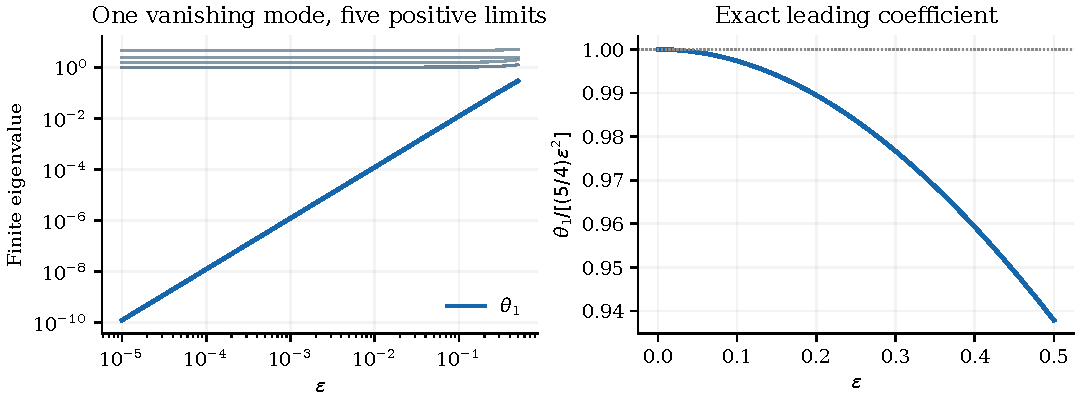
\includegraphics[width=.94\textwidth]{figures/output/six_modes.pdf}
\caption{Eigenvalues of the explicit finite form
\eqref{eq:balanced-finite-form}, before the factor $t^2\beta$.
Left: all six eigenvalues for positive $\varepsilon$, with the weak
mode emphasized. Right: its ratio to $(5/4)\varepsilon^2$.
At $\varepsilon=0$ that eigenvalue is exactly zero and the other
five remain positive. Passage to the trace-free HE spectrum is the relative
estimate in Theorem~\ref{thm:balanced-spectrum}, not a numerical
solution of the HE equation.}
\label{fig:six-modes}
\end{figure}

The balanced identities can also be checked without radicals.
Eliminate $e$ from \eqref{eq:z-identity}:
\[
 e=\frac{5z^2+2z-3}{4z+3}.
\]
Rational $z$ near $3/5$ gives exact rational data for the slope and
moment identities. The accompanying calculation verifies those identities,
the kernel dimensions, and the two first-variation coefficients.
These finite checks supplement the printed arguments; they do not
replace the analytic estimates.

\begin{figure}[htbp]
\centering
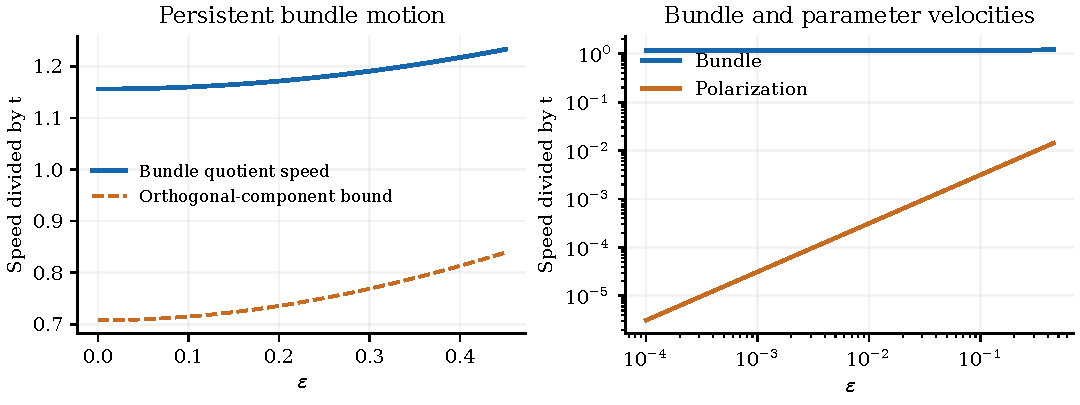
\includegraphics[width=.94\textwidth]{figures/output/curve_motion.pdf}
\caption{The cubic-rotation curve at $t=0.1$, computed in the finite
model. Left: the coefficient quotient speed divided by $t$, with
the explicit lower bound from \eqref{eq:curve-transverse-energy}.
Right: the polarization speed divided by $t$ and the bundle quotient
speed. The latter stays positive as the parameter speed tends to
zero. The actual bundle and total metric bounds follow from
\eqref{eq:curve-ks-lower} and Proposition~\ref{prop:total-metric}.}
\label{fig:curve-motion}
\end{figure}

Figure~\ref{fig:curve-motion} distinguishes the two sources of motion.
The polynomial direction $\dot P_\varepsilon$ remains perpendicular
to every finite orbit direction, whereas $p'(\varepsilon)=O(t^2\varepsilon)$.
This is why the nonzero bundle tangent persists in the parameter-inclusive
metric. The unrotated family has zero interior bundle tangent despite
its varying HE spectrum. The distinction is visible algebraically
before invoking any estimate on the actual metric.

\FloatBarrier
\begin{thebibliography}{Wue26c}

\bibitem[BiS16]{BiswasSchumacher16}
I.~Biswas and G.~Schumacher,
\emph{The Weil--Petersson current for moduli of vector bundles and applications to orbifolds},
Ann. Fac. Sci. Toulouse Math. (6) \textbf{25} (2016), no.~4, 895--917.
\href{https://doi.org/10.5802/afst.1514}{doi:10.5802/afst.1514}.

\bibitem[BuS20]{BuchdahlSchumacher20}
N.~Buchdahl and G.~Schumacher,
\emph{Polystability and the Hitchin--Kobayashi correspondence}, preprint (2020),
\href{https://arxiv.org/abs/2002.03548v1}{arXiv:2002.03548v1}.

\bibitem[CT24]{ClarkeTipler24}
A.~Clarke and C.~Tipler,
\emph{Semi-stability and local wall-crossing for Hermitian Yang--Mills connections},
J. Symplectic Geom. \textbf{22} (2024), no.~3, 673--694.
Locators refer to \href{https://arxiv.org/abs/2304.05245v1}{arXiv:2304.05245v1}.

\bibitem[Del25]{Delloque25}
R.~Delloque, \emph{Continuity of HYM connections with respect to metric variations},
J. London Math. Soc. (2) \textbf{112} (2025), no.~1, e70219.
\href{https://doi.org/10.1112/jlms.70219}{doi:10.1112/jlms.70219}.
Locators refer to \href{https://arxiv.org/abs/2403.16814v4}{arXiv:2403.16814v4}.

\bibitem[Kob87]{Kobayashi87}
S.~Kobayashi, \emph{Differential Geometry of Complex Vector Bundles},
Publications of the Mathematical Society of Japan, vol.~15,
Princeton University Press, Princeton, NJ, 1987.
\href{https://www.mathsoc.jp/assets/pdf/publications/pubmsj/Vol15.pdf}{Mathematical Society of Japan edition}.

\bibitem[Pal61]{Palais61}
R.~S.~Palais, \emph{On the existence of slices for actions of non-compact Lie groups},
Ann. of Math. (2) \textbf{73} (1961), no.~2, 295--323.
\href{https://doi.org/10.2307/1970335}{doi:10.2307/1970335}.

\bibitem[Stacks]{stacks}
The Stacks Project Authors, \emph{The Stacks Project},
\href{https://stacks.math.columbia.edu/tag/01XT}{Tag 01XT (projective-space cohomology)} and
\href{https://stacks.math.columbia.edu/tag/0BED}{Tag 0BED (K\"unneth formula)},
accessed October 31, 2026.

\bibitem[Wue26a]{WuebbenWallMetrics26}
B.~J.~Wuebben, \emph{$L^2$ metrics on Hermitian--Yang--Mills moduli spaces near a stability wall},
preprint, October 31, 2026.
\href{https://doi.org/10.5281/zenodo.23850992}{doi:10.5281/zenodo.23850992}.

\bibitem[Wue26b]{WuebbenRelativeMetrics26}
B.~J.~Wuebben, \emph{Relative metric estimates near reducible Yang--Mills connections},
preprint, October 28, 2026.
\href{https://doi.org/10.5281/zenodo.23740619}{doi:10.5281/zenodo.23740619}.

\bibitem[Wue26c]{WuebbenRepeated26}
B.~J.~Wuebben, \emph{Uniform Hermitian--Einstein spectra with repeated stable factors},
preprint, October 29, 2026.
\href{https://doi.org/10.5281/zenodo.23780241}{doi:10.5281/zenodo.23780241}.

\end{thebibliography}

\end{document}
